\documentclass{article}\usepackage[]{graphicx}\usepackage[]{color}
%% maxwidth is the original width if it is less than linewidth
%% otherwise use linewidth (to make sure the graphics do not exceed the margin)
\makeatletter
\def\maxwidth{ %
  \ifdim\Gin@nat@width>\linewidth
    \linewidth
  \else
    \Gin@nat@width
  \fi
}
\makeatother

\definecolor{fgcolor}{rgb}{0.345, 0.345, 0.345}
\newcommand{\hlnum}[1]{\textcolor[rgb]{0.686,0.059,0.569}{#1}}%
\newcommand{\hlstr}[1]{\textcolor[rgb]{0.192,0.494,0.8}{#1}}%
\newcommand{\hlcom}[1]{\textcolor[rgb]{0.678,0.584,0.686}{\textit{#1}}}%
\newcommand{\hlopt}[1]{\textcolor[rgb]{0,0,0}{#1}}%
\newcommand{\hlstd}[1]{\textcolor[rgb]{0.345,0.345,0.345}{#1}}%
\newcommand{\hlkwa}[1]{\textcolor[rgb]{0.161,0.373,0.58}{\textbf{#1}}}%
\newcommand{\hlkwb}[1]{\textcolor[rgb]{0.69,0.353,0.396}{#1}}%
\newcommand{\hlkwc}[1]{\textcolor[rgb]{0.333,0.667,0.333}{#1}}%
\newcommand{\hlkwd}[1]{\textcolor[rgb]{0.737,0.353,0.396}{\textbf{#1}}}%

\usepackage{framed}
\makeatletter
\newenvironment{kframe}{%
 \def\at@end@of@kframe{}%
 \ifinner\ifhmode%
  \def\at@end@of@kframe{\end{minipage}}%
  \begin{minipage}{\columnwidth}%
 \fi\fi%
 \def\FrameCommand##1{\hskip\@totalleftmargin \hskip-\fboxsep
 \colorbox{shadecolor}{##1}\hskip-\fboxsep
     % There is no \\@totalrightmargin, so:
     \hskip-\linewidth \hskip-\@totalleftmargin \hskip\columnwidth}%
 \MakeFramed {\advance\hsize-\width
   \@totalleftmargin\z@ \linewidth\hsize
   \@setminipage}}%
 {\par\unskip\endMakeFramed%
 \at@end@of@kframe}
\makeatother

\definecolor{shadecolor}{rgb}{.97, .97, .97}
\definecolor{messagecolor}{rgb}{0, 0, 0}
\definecolor{warningcolor}{rgb}{1, 0, 1}
\definecolor{errorcolor}{rgb}{1, 0, 0}
\newenvironment{knitrout}{}{} % an empty environment to be redefined in TeX

\usepackage{alltt}
\usepackage{graphicx}
\usepackage[left=1.00in, right=1.00in, top=1.00in, bottom=1.00in]{geometry}
\usepackage{hyperref}

\hypersetup{
    colorlinks,
    citecolor=black,
    filecolor=black,
    linkcolor=blue,
    urlcolor=black
}

\DeclareGraphicsExtensions{.png,.jpg}

\title{Appendix and Model Output Plots}
\author{Daniel Chen \\ Mailman School of Public health \\ Columbia University}
\date{}



\IfFileExists{upquote.sty}{\usepackage{upquote}}{}

\begin{document}
\maketitle
\tableofcontents

\newpage

\section{Plotting Function}
\label{sec:plot-function}
For the plots, x-axis is time, y-axis is processing unit activation value

\begin{knitrout}
\definecolor{shadecolor}{rgb}{0.969, 0.969, 0.969}\color{fgcolor}\begin{kframe}
\begin{alltt}
\hlstd{plot.thesis.data} \hlkwb{<-} \hlkwa{function}\hlstd{(}\hlkwc{data}\hlstd{,} \hlkwc{numAgents}\hlstd{,} \hlkwc{numTimeTicks}\hlstd{,} \hlkwc{subx} \hlstd{=} \hlnum{0}\hlstd{,} \hlkwc{xmin} \hlstd{=} \hlnum{0}\hlstd{,}
    \hlkwc{xmax} \hlstd{=} \hlnum{10}\hlstd{) \{}
    \hlcom{# Takes a CSV from my thesis output, assign's column names, converts}
    \hlcom{# processing unit values into numerics plots the average activation value}
    \hlcom{# for each processing unit for each agent in each time tick Args: data:}
    \hlcom{# String value of the directory and file of CSV numAgents: Number of agents}
    \hlcom{# ran in the simulation of the CSV numTimeTicks: Number of time ticks ran in}
    \hlcom{# the simulation of the CSV subx: defaults to 0, used to section regions of}
    \hlcom{# the x axis, 0 for no sub-sectioning, 1 for yes sub-sectioning xmin:}
    \hlcom{# defaults to 0, the lower bound of the x-axis if subx is 1 xmax: defaults}
    \hlcom{# to 0, the upper bound of the x-axis if subx is 1 Returns: Line graph}

    \hlcom{# Load data}
    \hlstd{x} \hlkwb{<-} \hlkwd{read.csv}\hlstd{(data,} \hlkwc{header} \hlstd{=} \hlnum{FALSE}\hlstd{,} \hlkwc{stringsAsFactors} \hlstd{=} \hlnum{FALSE}\hlstd{)}

    \hlcom{# Rename dataframe column names}
    \hlkwd{names}\hlstd{(x)} \hlkwb{<-} \hlkwd{c}\hlstd{(}\hlstr{"time"}\hlstd{,} \hlstr{"agent"}\hlstd{,} \hlstr{"p1"}\hlstd{,} \hlstr{"p2"}\hlstd{,} \hlstr{"p3"}\hlstd{,} \hlstr{"p4"}\hlstd{,} \hlstr{"p5"}\hlstd{,} \hlstr{"n1"}\hlstd{,} \hlstr{"n2"}\hlstd{,}
        \hlstr{"n3"}\hlstd{,} \hlstr{"n4"}\hlstd{,} \hlstr{"n5"}\hlstd{)}

    \hlcom{# Convert string factors into numerics}
    \hlkwa{for} \hlstd{(i} \hlkwa{in} \hlnum{3}\hlopt{:}\hlnum{12}\hlstd{) \{}
        \hlstd{x[, i]} \hlkwb{<-} \hlkwd{as.numeric}\hlstd{(x[, i])}
    \hlstd{\}}

    \hlstd{x.1} \hlkwb{<-} \hlstd{x[}\hlkwd{seq}\hlstd{(}\hlnum{1}\hlstd{, numTimeTicks} \hlopt{*} \hlstd{numAgents, numAgents), ]}
    \hlstd{x.2} \hlkwb{<-} \hlstd{x[}\hlkwd{seq}\hlstd{(}\hlnum{2}\hlstd{, numTimeTicks} \hlopt{*} \hlstd{numAgents, numAgents), ]}
    \hlstd{x.3} \hlkwb{<-} \hlstd{x[}\hlkwd{seq}\hlstd{(}\hlnum{3}\hlstd{, numTimeTicks} \hlopt{*} \hlstd{numAgents, numAgents), ]}
    \hlstd{x.4} \hlkwb{<-} \hlstd{x[}\hlkwd{seq}\hlstd{(}\hlnum{4}\hlstd{, numTimeTicks} \hlopt{*} \hlstd{numAgents, numAgents), ]}
    \hlstd{x.5} \hlkwb{<-} \hlstd{x[}\hlkwd{seq}\hlstd{(}\hlnum{5}\hlstd{, numTimeTicks} \hlopt{*} \hlstd{numAgents, numAgents), ]}

    \hlstd{x.1.ave.pos} \hlkwb{<-} \hlkwd{apply}\hlstd{(x.1[,} \hlkwd{c}\hlstd{(}\hlnum{3}\hlstd{,} \hlnum{4}\hlstd{,} \hlnum{5}\hlstd{,} \hlnum{6}\hlstd{,} \hlnum{7}\hlstd{)],} \hlnum{1}\hlstd{, mean)}
    \hlstd{x.1.ave.neg} \hlkwb{<-} \hlkwd{apply}\hlstd{(x.1[,} \hlkwd{c}\hlstd{(}\hlnum{8}\hlstd{,} \hlnum{9}\hlstd{,} \hlnum{10}\hlstd{,} \hlnum{11}\hlstd{,} \hlnum{12}\hlstd{)],} \hlnum{1}\hlstd{, mean)}

    \hlstd{x.2.ave.pos} \hlkwb{<-} \hlkwd{apply}\hlstd{(x.2[,} \hlkwd{c}\hlstd{(}\hlnum{3}\hlstd{,} \hlnum{4}\hlstd{,} \hlnum{5}\hlstd{,} \hlnum{6}\hlstd{,} \hlnum{7}\hlstd{)],} \hlnum{1}\hlstd{, mean)}
    \hlstd{x.2.ave.neg} \hlkwb{<-} \hlkwd{apply}\hlstd{(x.2[,} \hlkwd{c}\hlstd{(}\hlnum{8}\hlstd{,} \hlnum{9}\hlstd{,} \hlnum{10}\hlstd{,} \hlnum{11}\hlstd{,} \hlnum{12}\hlstd{)],} \hlnum{1}\hlstd{, mean)}

    \hlstd{x.3.ave.pos} \hlkwb{<-} \hlkwd{apply}\hlstd{(x.3[,} \hlkwd{c}\hlstd{(}\hlnum{3}\hlstd{,} \hlnum{4}\hlstd{,} \hlnum{5}\hlstd{,} \hlnum{6}\hlstd{,} \hlnum{7}\hlstd{)],} \hlnum{1}\hlstd{, mean)}
    \hlstd{x.3.ave.neg} \hlkwb{<-} \hlkwd{apply}\hlstd{(x.3[,} \hlkwd{c}\hlstd{(}\hlnum{8}\hlstd{,} \hlnum{9}\hlstd{,} \hlnum{10}\hlstd{,} \hlnum{11}\hlstd{,} \hlnum{12}\hlstd{)],} \hlnum{1}\hlstd{, mean)}

    \hlstd{x.4.ave.pos} \hlkwb{<-} \hlkwd{apply}\hlstd{(x.4[,} \hlkwd{c}\hlstd{(}\hlnum{3}\hlstd{,} \hlnum{4}\hlstd{,} \hlnum{5}\hlstd{,} \hlnum{6}\hlstd{,} \hlnum{7}\hlstd{)],} \hlnum{1}\hlstd{, mean)}
    \hlstd{x.4.ave.neg} \hlkwb{<-} \hlkwd{apply}\hlstd{(x.4[,} \hlkwd{c}\hlstd{(}\hlnum{8}\hlstd{,} \hlnum{9}\hlstd{,} \hlnum{10}\hlstd{,} \hlnum{11}\hlstd{,} \hlnum{12}\hlstd{)],} \hlnum{1}\hlstd{, mean)}

    \hlstd{x.5.ave.pos} \hlkwb{<-} \hlkwd{apply}\hlstd{(x.5[,} \hlkwd{c}\hlstd{(}\hlnum{3}\hlstd{,} \hlnum{4}\hlstd{,} \hlnum{5}\hlstd{,} \hlnum{6}\hlstd{,} \hlnum{7}\hlstd{)],} \hlnum{1}\hlstd{, mean)}
    \hlstd{x.5.ave.neg} \hlkwb{<-} \hlkwd{apply}\hlstd{(x.5[,} \hlkwd{c}\hlstd{(}\hlnum{8}\hlstd{,} \hlnum{9}\hlstd{,} \hlnum{10}\hlstd{,} \hlnum{11}\hlstd{,} \hlnum{12}\hlstd{)],} \hlnum{1}\hlstd{, mean)}

    \hlkwa{if} \hlstd{(subx} \hlopt{==} \hlnum{0}\hlstd{) \{}
        \hlcom{# print(head(x, numAgents)) print(tail(x, numAgents))}

        \hlkwd{plot}\hlstd{(x.1.ave.pos,} \hlkwc{lty} \hlstd{=} \hlnum{1}\hlstd{,} \hlkwc{col} \hlstd{=} \hlnum{1}\hlstd{,} \hlkwc{type} \hlstd{=} \hlstr{"b"}\hlstd{,} \hlkwc{ylim} \hlstd{=} \hlkwd{c}\hlstd{(}\hlnum{0}\hlstd{,} \hlnum{1}\hlstd{))}
        \hlkwd{lines}\hlstd{(x.1.ave.neg,} \hlkwc{lty} \hlstd{=} \hlnum{2}\hlstd{,} \hlkwc{col} \hlstd{=} \hlnum{1}\hlstd{,} \hlkwc{type} \hlstd{=} \hlstr{"b"}\hlstd{,} \hlkwc{lwd} \hlstd{=} \hlnum{3}\hlstd{)}

        \hlkwd{lines}\hlstd{(x.2.ave.neg,} \hlkwc{ylim} \hlstd{=} \hlkwd{c}\hlstd{(}\hlnum{0}\hlstd{,} \hlnum{1}\hlstd{),} \hlkwc{lty} \hlstd{=} \hlnum{1}\hlstd{,} \hlkwc{col} \hlstd{=} \hlnum{2}\hlstd{,} \hlkwc{type} \hlstd{=} \hlstr{"b"}\hlstd{)}
        \hlkwd{lines}\hlstd{(x.2.ave.neg,} \hlkwc{lty} \hlstd{=} \hlnum{2}\hlstd{,} \hlkwc{col} \hlstd{=} \hlnum{2}\hlstd{,} \hlkwc{type} \hlstd{=} \hlstr{"b"}\hlstd{,} \hlkwc{lwd} \hlstd{=} \hlnum{3}\hlstd{)}

        \hlkwd{lines}\hlstd{(x.3.ave.neg,} \hlkwc{lty} \hlstd{=} \hlnum{1}\hlstd{,} \hlkwc{col} \hlstd{=} \hlnum{3}\hlstd{,} \hlkwc{type} \hlstd{=} \hlstr{"b"}\hlstd{)}
        \hlkwd{lines}\hlstd{(x.3.ave.neg,} \hlkwc{lty} \hlstd{=} \hlnum{2}\hlstd{,} \hlkwc{col} \hlstd{=} \hlnum{3}\hlstd{,} \hlkwc{type} \hlstd{=} \hlstr{"b"}\hlstd{,} \hlkwc{lwd} \hlstd{=} \hlnum{3}\hlstd{)}

        \hlkwd{lines}\hlstd{(x.4.ave.neg,} \hlkwc{lty} \hlstd{=} \hlnum{1}\hlstd{,} \hlkwc{col} \hlstd{=} \hlnum{4}\hlstd{,} \hlkwc{type} \hlstd{=} \hlstr{"b"}\hlstd{)}
        \hlkwd{lines}\hlstd{(x.4.ave.neg,} \hlkwc{lty} \hlstd{=} \hlnum{2}\hlstd{,} \hlkwc{col} \hlstd{=} \hlnum{4}\hlstd{,} \hlkwc{type} \hlstd{=} \hlstr{"b"}\hlstd{,} \hlkwc{lwd} \hlstd{=} \hlnum{3}\hlstd{)}

        \hlkwd{lines}\hlstd{(x.5.ave.neg,} \hlkwc{lty} \hlstd{=} \hlnum{1}\hlstd{,} \hlkwc{col} \hlstd{=} \hlnum{5}\hlstd{,} \hlkwc{type} \hlstd{=} \hlstr{"b"}\hlstd{)}
        \hlkwd{lines}\hlstd{(x.5.ave.neg,} \hlkwc{lty} \hlstd{=} \hlnum{2}\hlstd{,} \hlkwc{col} \hlstd{=} \hlnum{5}\hlstd{,} \hlkwc{type} \hlstd{=} \hlstr{"b"}\hlstd{,} \hlkwc{lwd} \hlstd{=} \hlnum{3}\hlstd{)}
    \hlstd{\}}

    \hlkwa{if} \hlstd{(subx} \hlopt{==} \hlnum{1}\hlstd{) \{}
        \hlcom{# print(head(x, numAgents)) print(tail(x, numAgents))}

        \hlkwd{plot}\hlstd{(x.1.ave.pos,} \hlkwc{lty} \hlstd{=} \hlnum{1}\hlstd{,} \hlkwc{col} \hlstd{=} \hlnum{1}\hlstd{,} \hlkwc{type} \hlstd{=} \hlstr{"b"}\hlstd{,} \hlkwc{ylim} \hlstd{=} \hlkwd{c}\hlstd{(}\hlnum{0}\hlstd{,} \hlnum{1}\hlstd{),} \hlkwc{xlim} \hlstd{=} \hlkwd{c}\hlstd{(xmin,}
            \hlstd{xmax))}
        \hlkwd{lines}\hlstd{(x.1.ave.neg,} \hlkwc{lty} \hlstd{=} \hlnum{2}\hlstd{,} \hlkwc{col} \hlstd{=} \hlnum{1}\hlstd{,} \hlkwc{type} \hlstd{=} \hlstr{"b"}\hlstd{,} \hlkwc{lwd} \hlstd{=} \hlnum{3}\hlstd{)}

        \hlkwd{lines}\hlstd{(x.2.ave.neg,} \hlkwc{ylim} \hlstd{=} \hlkwd{c}\hlstd{(}\hlnum{0}\hlstd{,} \hlnum{1}\hlstd{),} \hlkwc{lty} \hlstd{=} \hlnum{1}\hlstd{,} \hlkwc{col} \hlstd{=} \hlnum{2}\hlstd{,} \hlkwc{type} \hlstd{=} \hlstr{"b"}\hlstd{)}
        \hlkwd{lines}\hlstd{(x.2.ave.neg,} \hlkwc{lty} \hlstd{=} \hlnum{2}\hlstd{,} \hlkwc{col} \hlstd{=} \hlnum{2}\hlstd{,} \hlkwc{type} \hlstd{=} \hlstr{"b"}\hlstd{,} \hlkwc{lwd} \hlstd{=} \hlnum{3}\hlstd{)}

        \hlkwd{lines}\hlstd{(x.3.ave.neg,} \hlkwc{lty} \hlstd{=} \hlnum{1}\hlstd{,} \hlkwc{col} \hlstd{=} \hlnum{3}\hlstd{,} \hlkwc{type} \hlstd{=} \hlstr{"b"}\hlstd{)}
        \hlkwd{lines}\hlstd{(x.3.ave.neg,} \hlkwc{lty} \hlstd{=} \hlnum{2}\hlstd{,} \hlkwc{col} \hlstd{=} \hlnum{3}\hlstd{,} \hlkwc{type} \hlstd{=} \hlstr{"b"}\hlstd{,} \hlkwc{lwd} \hlstd{=} \hlnum{3}\hlstd{)}

        \hlkwd{lines}\hlstd{(x.4.ave.neg,} \hlkwc{lty} \hlstd{=} \hlnum{1}\hlstd{,} \hlkwc{col} \hlstd{=} \hlnum{4}\hlstd{,} \hlkwc{type} \hlstd{=} \hlstr{"b"}\hlstd{)}
        \hlkwd{lines}\hlstd{(x.4.ave.neg,} \hlkwc{lty} \hlstd{=} \hlnum{2}\hlstd{,} \hlkwc{col} \hlstd{=} \hlnum{4}\hlstd{,} \hlkwc{type} \hlstd{=} \hlstr{"b"}\hlstd{,} \hlkwc{lwd} \hlstd{=} \hlnum{3}\hlstd{)}

        \hlkwd{lines}\hlstd{(x.5.ave.neg,} \hlkwc{lty} \hlstd{=} \hlnum{1}\hlstd{,} \hlkwc{col} \hlstd{=} \hlnum{5}\hlstd{,} \hlkwc{type} \hlstd{=} \hlstr{"b"}\hlstd{)}
        \hlkwd{lines}\hlstd{(x.5.ave.neg,} \hlkwc{lty} \hlstd{=} \hlnum{2}\hlstd{,} \hlkwc{col} \hlstd{=} \hlnum{5}\hlstd{,} \hlkwc{type} \hlstd{=} \hlstr{"b"}\hlstd{,} \hlkwc{lwd} \hlstd{=} \hlnum{3}\hlstd{)}
    \hlstd{\}}
\hlstd{\}}
\end{alltt}
\end{kframe}
\end{knitrout}


\newpage

\section{Sanity Checks}
\label{sec:sanity-checks}

\subsection{Sanity Check 1}
\label{sec:sanity1}
Sanity Case:
\begin{itemize}
  \item Agents Activated: Agent 1 ont
  \item Valence Bank: positive only
  \begin{itemize}
      \item Valence bank activation: 1's
  \end{itemize}
  \item Valence bank Weights: random
  \begin{itemize}
      \item opposite 0
      \item corresponding 0
      \item carry over = 0.2
      \item bias = 0
      \item decay = -0.5
  \end{itemize}
  \item Network: circle
\end{itemize}

%
% \newpage
% <<plot-sanity-1, fig.cap="Sanity Checking 1", fig.show='asis'>>=
% plot.thesis.data("/home/dchen/git/repast-neural-network-agent-based-model/R/data/agent1pos1.csv",
%   10, 10)
% @
%
% \newpage
% \subsubsection{Sanity 1}
% <<plot-sanity1-v2, fig.cap="Sanity 1 with re-implemented edge list", fig.show='asis'>>=
% plot.thesis.data("/home/dchen/git/repast-neural-network-agent-based-model/R/data/sanity1-new-external.csv", 10, 10)
% @

\newpage
\subsubsection{Sanity 1, no step}
\begin{knitrout}
\definecolor{shadecolor}{rgb}{0.969, 0.969, 0.969}\color{fgcolor}\begin{kframe}
\begin{alltt}
\hlkwd{plot.thesis.data}\hlstd{(}\hlstr{"/home/dchen/git/repast-neural-network-agent-based-model/R/data/sanity1-new-external-no-step.csv"}\hlstd{,}
    \hlnum{10}\hlstd{,} \hlnum{10}\hlstd{)}
\end{alltt}
\end{kframe}\begin{figure}[]

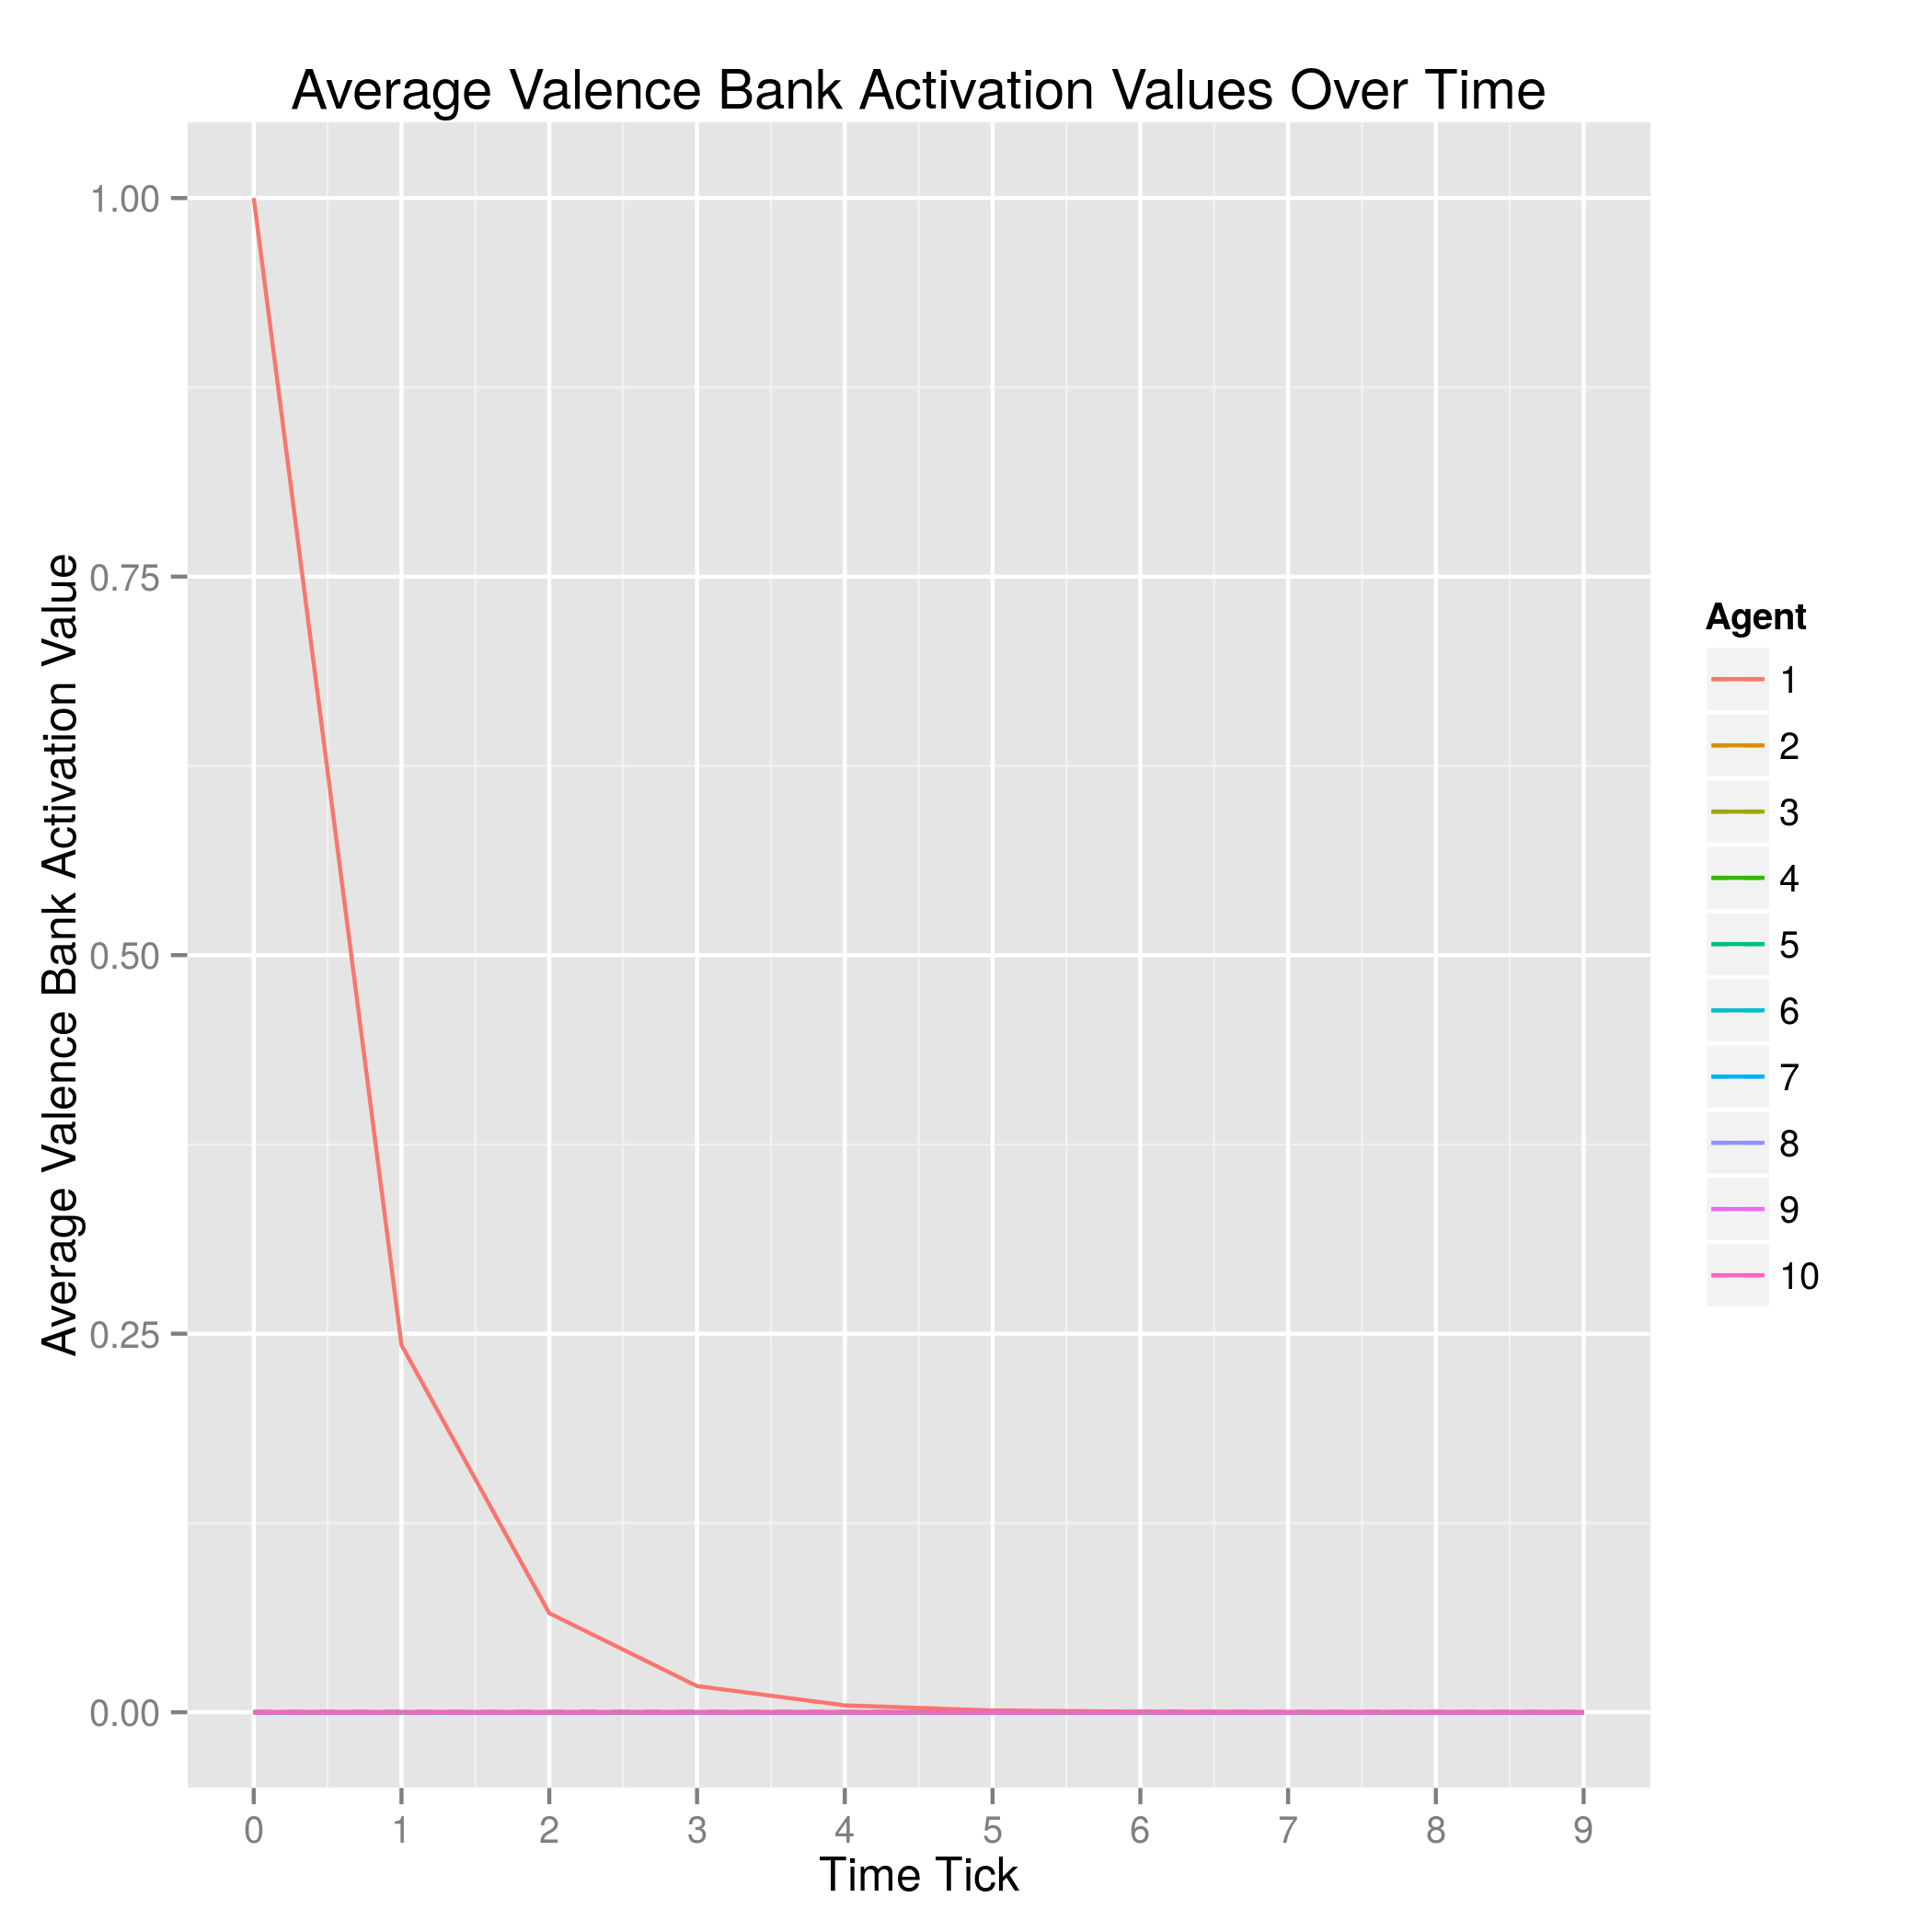
\includegraphics[width=\maxwidth]{figure/plot-sanity1-v2-nostep} \caption[Sanity 1 with re-implemented edge list, no step]{Sanity 1 with re-implemented edge list, no step\label{fig:plot-sanity1-v2-nostep}}
\end{figure}


\end{knitrout}


\newpage
\subsection{Sanity Check 2}
\label{sec:sanity2}
Sanity Case:
\begin{itemize}
  \item Agents Activated: Agent 1 ont
  \item Valence Bank: positive only
  \begin{itemize}
      \item Valence bank activation: \textbf{random}
  \end{itemize}
  \item Valence bank Weights: random
  \begin{itemize}
      \item opposite 0
      \item corresponding 0
      \item carry over = 0.2
      \item bias = 0
      \item decay = -0.5
  \end{itemize}
  \item Network: circle
\end{itemize}
%
% \newpage
% <<plot-sanity-2, fig.cap="Sanity Checking 2", fig.show='asis'>>=
% plot.thesis.data("/home/dchen/git/repast-neural-network-agent-based-model/R/data/agent1posrandom.csv", 10, 10)
% @
%
% \newpage
% \subsubsection{Sanity 2}
% <<plot-sanity-2-v2, fig.cap="Sanity Checking 2 with re-implemented edge list", fig.show='asis'>>=
% plot.thesis.data("/home/dchen/git/repast-neural-network-agent-based-model/R/data/sanity2-new-external.csv", 10, 10)
% @

\newpage
\subsubsection{Sanity 2, no step}
\begin{knitrout}
\definecolor{shadecolor}{rgb}{0.969, 0.969, 0.969}\color{fgcolor}\begin{kframe}
\begin{alltt}
\hlkwd{plot.thesis.data}\hlstd{(}\hlstr{"/home/dchen/git/repast-neural-network-agent-based-model/R/data/sanity2-new-external-no-step.csv"}\hlstd{,}
    \hlnum{10}\hlstd{,} \hlnum{10}\hlstd{)}
\end{alltt}
\end{kframe}\begin{figure}[]

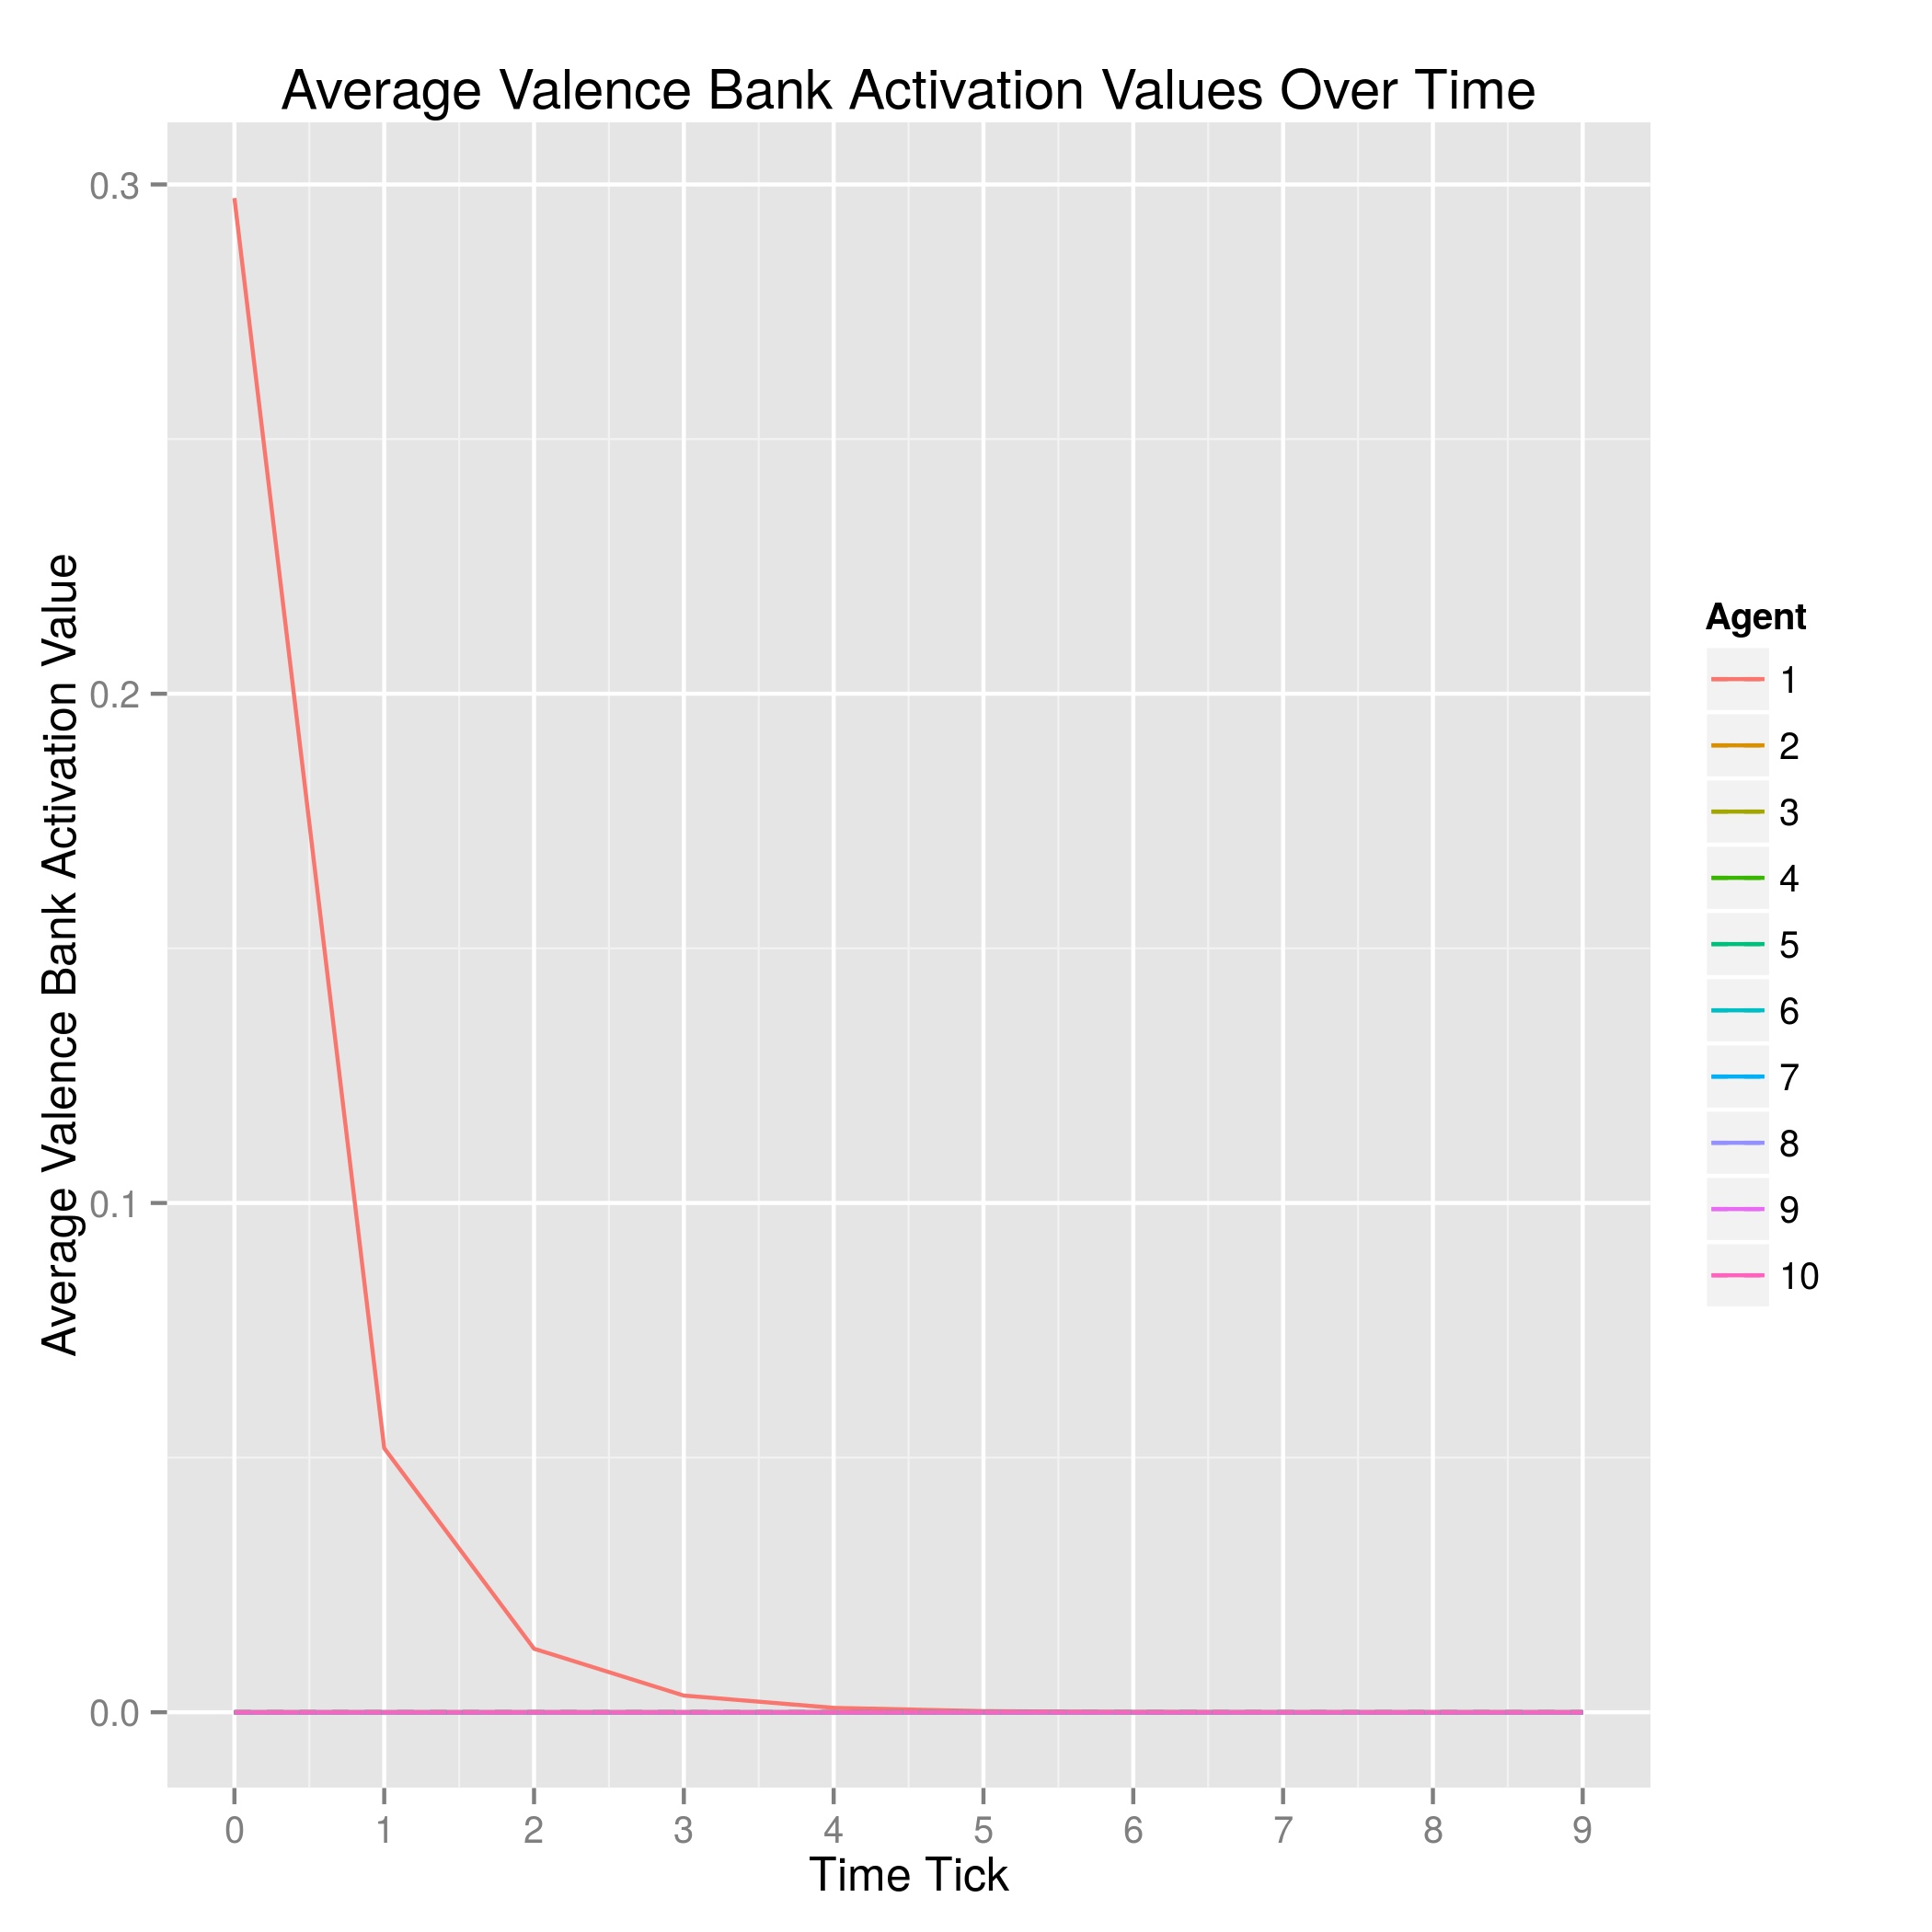
\includegraphics[width=\maxwidth]{figure/plot-sanity-2-v2-nostep} \caption[Sanity Checking 2 with re-implemented edge list, no step]{Sanity Checking 2 with re-implemented edge list, no step\label{fig:plot-sanity-2-v2-nostep}}
\end{figure}


\end{knitrout}


\newpage
\subsection{Sanity Check 3}
\label{sec:sanity3}
Sanity Case:
\begin{itemize}
  \item Agents Activated: Agent 1 ont
  \item Valence Bank: \textbf{both}
  \begin{itemize}
      \item Valence bank activation: random
  \end{itemize}
  \item Valence bank Weights: random
  \begin{itemize}
      \item opposite 0
      \item corresponding 0
      \item carry over = 0.2
      \item bias = 0
      \item decay = -0.5
  \end{itemize}
  \item Network: circle
\end{itemize}
%
% \newpage
% <<plot-sanity-3, fig.cap="Sanity Checking 3", fig.show='asis'>>=
% plot.thesis.data("/home/dchen/git/repast-neural-network-agent-based-model/R/data/agent1bothrandom.csv", 10, 10)
% @
%
% \newpage
% \subsubsection{Sanity 3}
% <<plot-sanity-3-v2, fig.cap="Sanity Checking 3 with re-implemented edge list", fig.show='asis'>>=
% plot.thesis.data("/home/dchen/git/repast-neural-network-agent-based-model/R/data/sanity3-new-external.csv", 10, 10)
% @

\newpage
\subsubsection{Sanity 3, no step}
\begin{knitrout}
\definecolor{shadecolor}{rgb}{0.969, 0.969, 0.969}\color{fgcolor}\begin{kframe}
\begin{alltt}
\hlkwd{plot.thesis.data}\hlstd{(}\hlstr{"/home/dchen/git/repast-neural-network-agent-based-model/R/data/sanity3-new-external-no-step.csv"}\hlstd{,}
    \hlnum{10}\hlstd{,} \hlnum{10}\hlstd{)}
\end{alltt}
\end{kframe}\begin{figure}[]

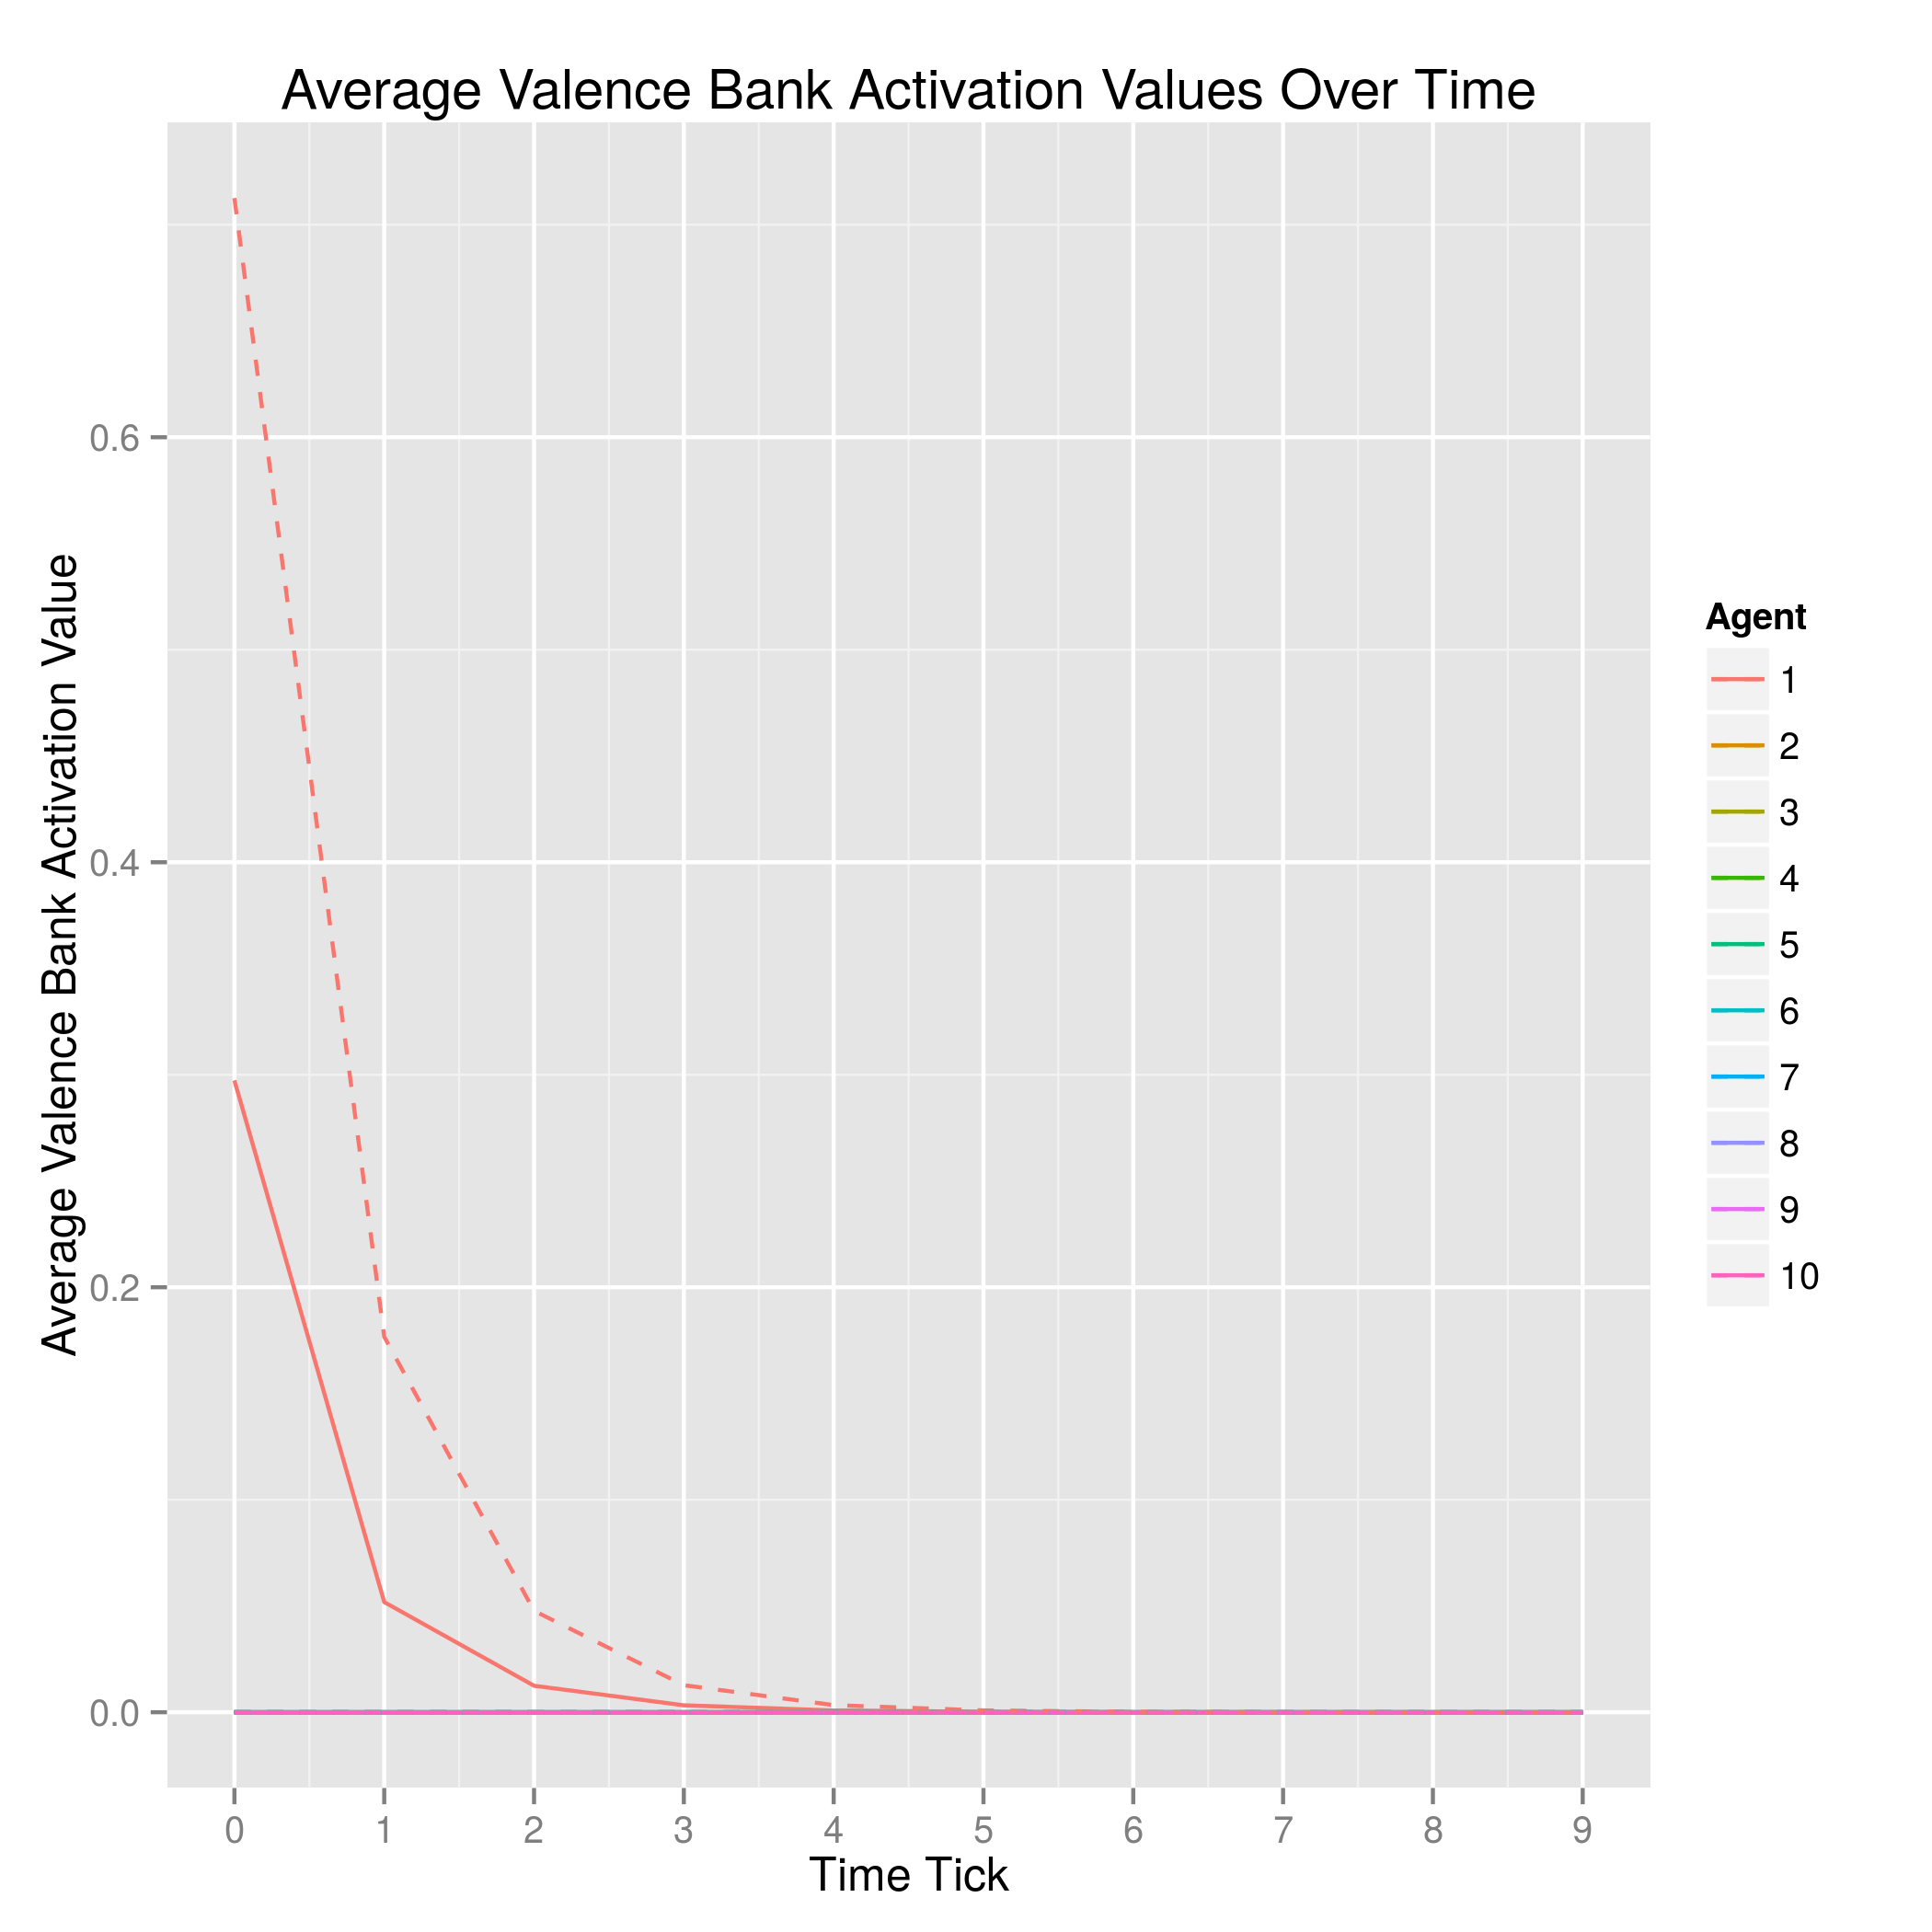
\includegraphics[width=\maxwidth]{figure/plot-sanity-3-v2-nostep} \caption[Sanity Checking 3 with re-implemented edge list, no step]{Sanity Checking 3 with re-implemented edge list, no step\label{fig:plot-sanity-3-v2-nostep}}
\end{figure}


\end{knitrout}


\newpage
\subsection{Sanity Check 4}
\label{sec:sanity4}
Sanity Case:
\begin{itemize}
  \item Agents Activated: Agent 1 ont
  \item Valence Bank: both
  \begin{itemize}
      \item Valence bank activation: random
  \end{itemize}
  \item Valence bank Weights: random
  \begin{itemize}
      \item opposite \textbf{-0.2}
      \item corresponding \textbf{0.5}
      \item carry over = 0.2
      \item bias = 0
      \item decay = -0.5
  \end{itemize}
  \item Network: circle
\end{itemize}
%
% \newpage
% <<plot-sanity-4, fig.cap="Sanity Checking 4", fig.show='asis'>>=
% plot.thesis.data("/home/dchen/git/repast-neural-network-agent-based-model/R/data/agent1bothrandom-weights.csv", 10, 10)
% @
%
% \newpage
% \subsubsection{Sanity 4}
% <<plot-sanity-4-v2, fig.cap="Sanity Checking 4 with re-implemented edge list", fig.show='asis'>>=
% plot.thesis.data("/home/dchen/git/repast-neural-network-agent-based-model/R/data/sanity4-new-external.csv", 10, 10)
% @

\newpage
\subsubsection{Sanity 4, no step}
\begin{knitrout}
\definecolor{shadecolor}{rgb}{0.969, 0.969, 0.969}\color{fgcolor}\begin{kframe}
\begin{alltt}
\hlkwd{plot.thesis.data}\hlstd{(}\hlstr{"/home/dchen/git/repast-neural-network-agent-based-model/R/data/sanity4-new-external-no-step.csv"}\hlstd{,}
    \hlnum{10}\hlstd{,} \hlnum{10}\hlstd{)}
\end{alltt}
\end{kframe}\begin{figure}[]

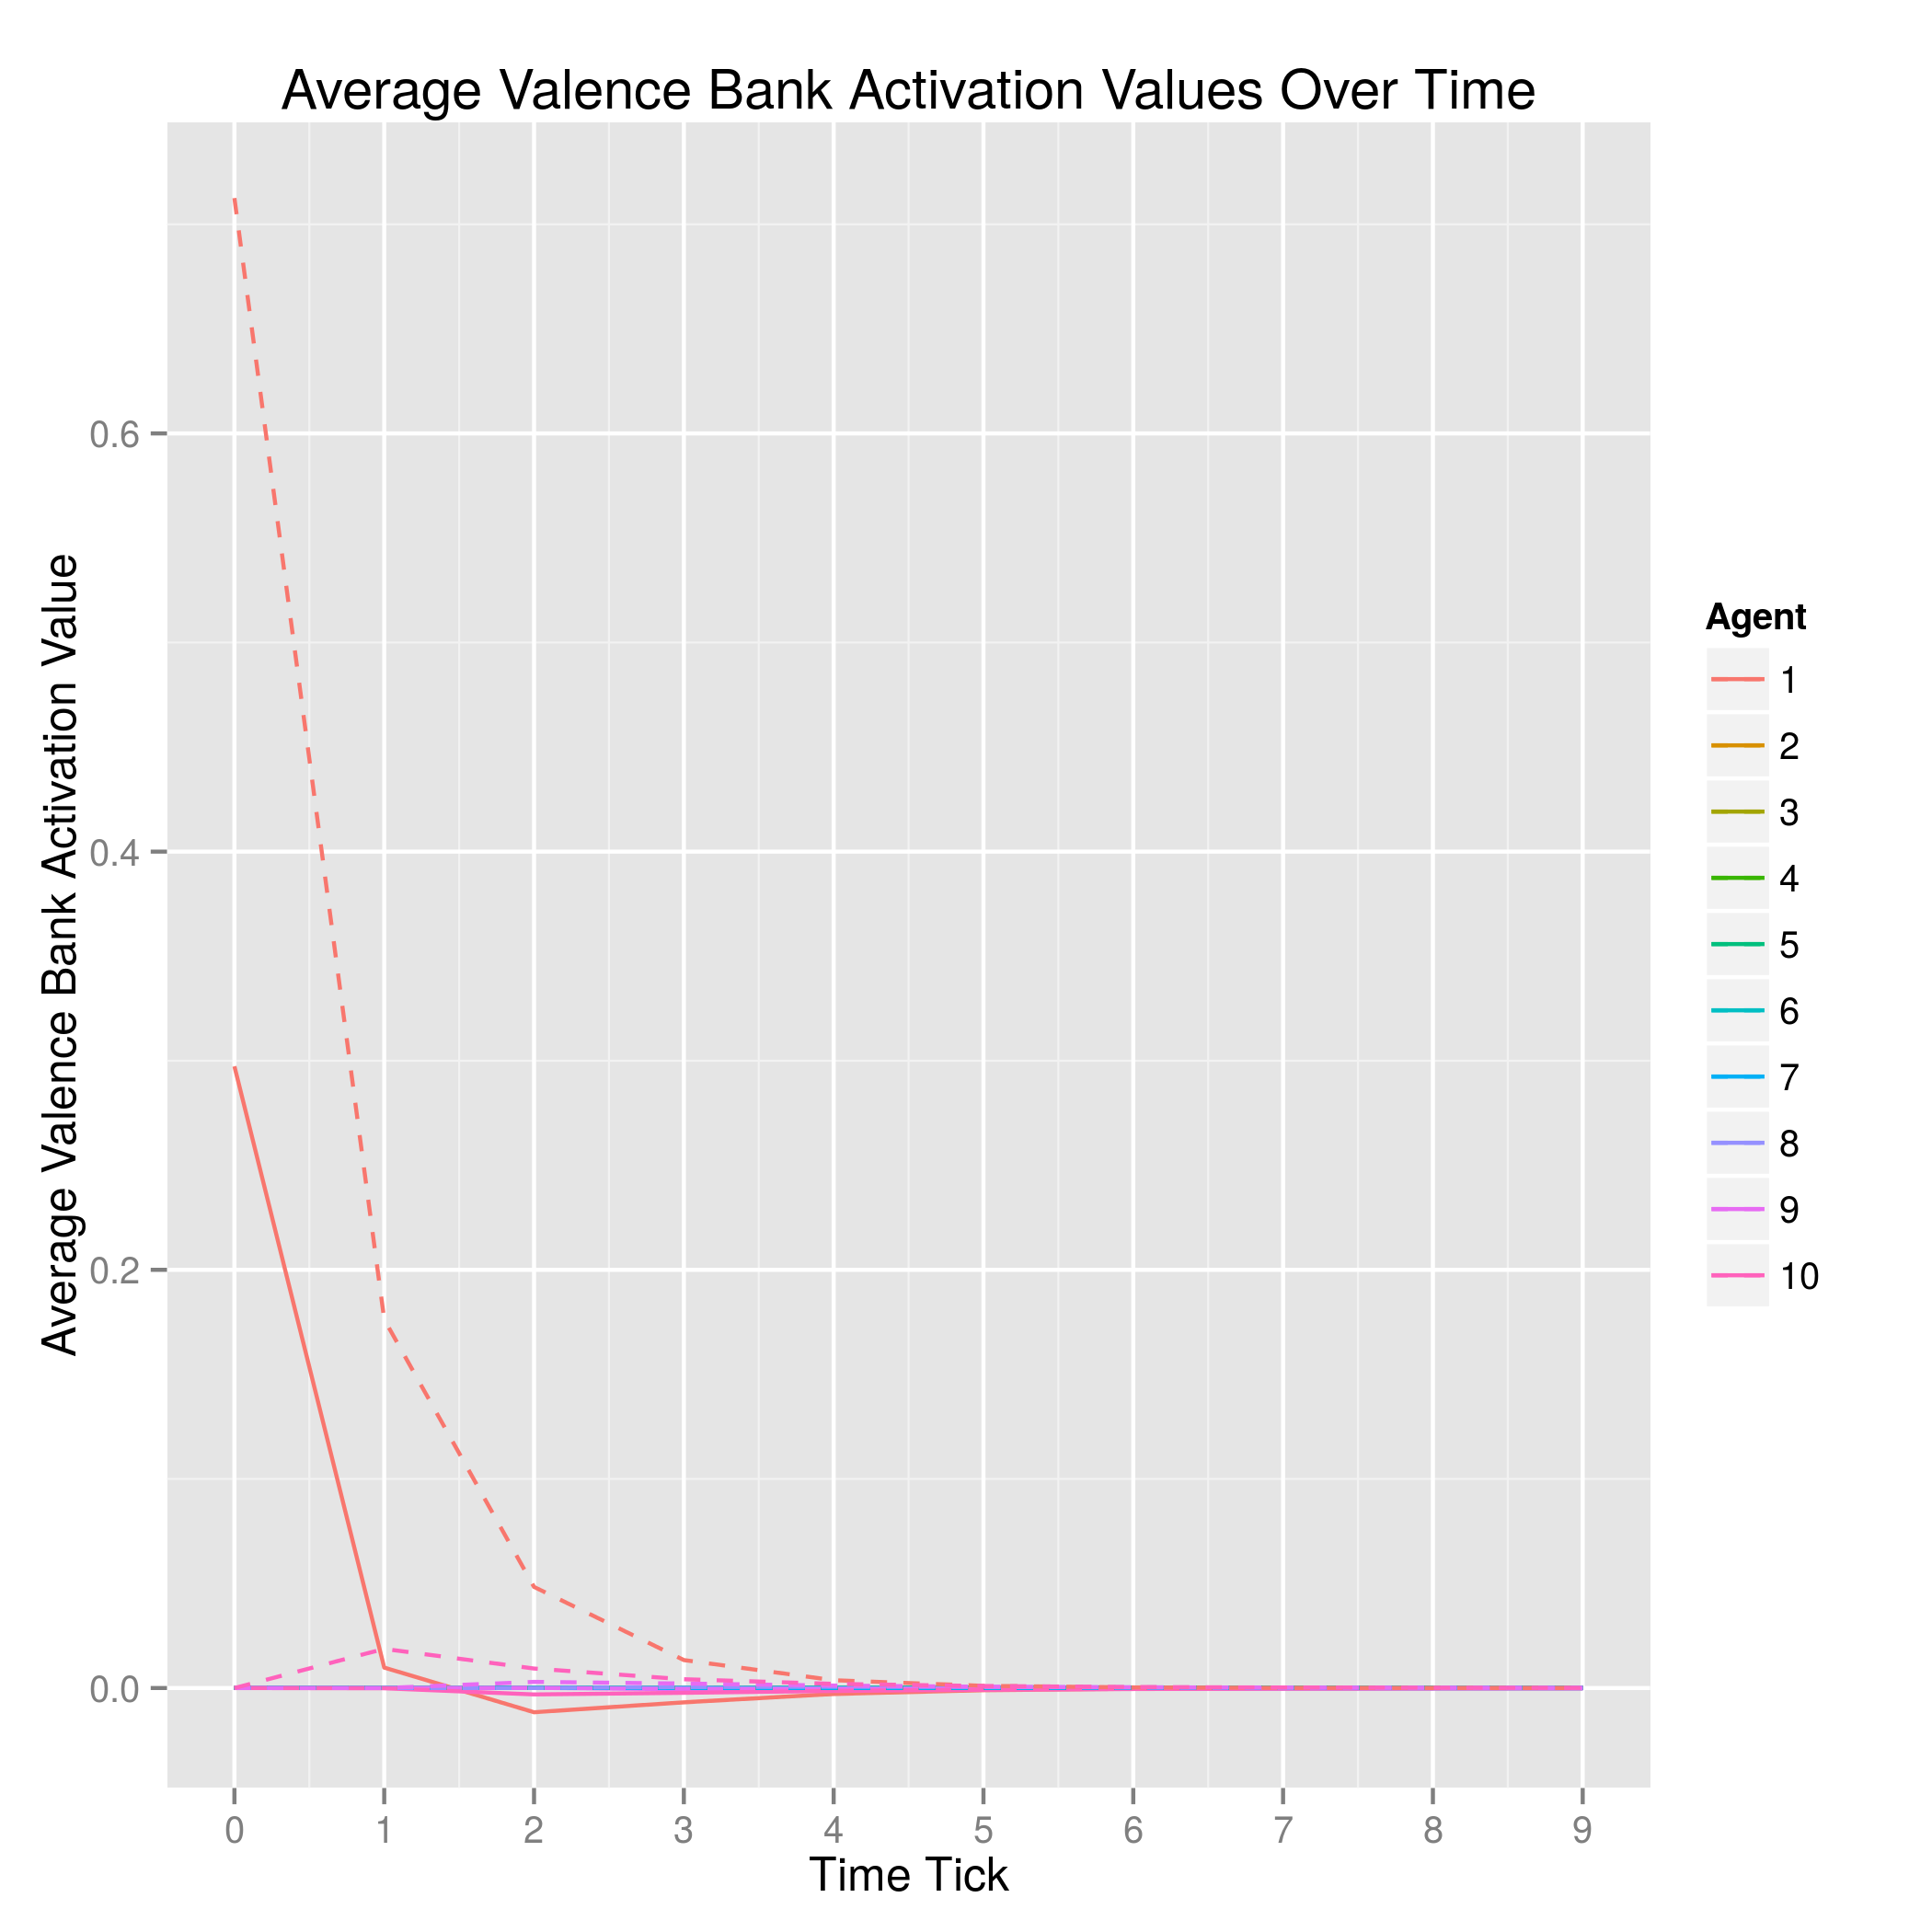
\includegraphics[width=\maxwidth]{figure/plot-sanity-4-v2-nostep} \caption[Sanity Checking 4 with re-implemented edge list, no step]{Sanity Checking 4 with re-implemented edge list, no step\label{fig:plot-sanity-4-v2-nostep}}
\end{figure}


\end{knitrout}


\newpage
\subsection{Sanity Check 5}
\label{sec:sanity5}
Sanity Case:
\begin{itemize}
  \item Agents Activated: \textbf{All}
  \item Valence Bank: both
  \begin{itemize}
      \item Valence bank activation: random
  \end{itemize}
  \item Valence bank Weights: random
  \begin{itemize}
      \item opposite -0.2
      \item corresponding 0.5
      \item carry over = 0.2
      \item bias = 0
      \item decay = -0.5
  \end{itemize}
  \item Network: circle
\end{itemize}
%
% \newpage
% <<plot-sanity-5, fig.cap="Sanity Checking 5", fig.show='asis'>>=
% plot.thesis.data("/home/dchen/git/repast-neural-network-agent-based-model/R/data/randomvaluesetweight.csv", 10, 10)
% @
%
% \newpage
% \subsubsection{Sanity 5}
% <<plot-sanity-5-v2, fig.cap="Sanity Checking 5 with re-implemented edge list", fig.show='asis'>>=
% plot.thesis.data("/home/dchen/git/repast-neural-network-agent-based-model/R/data/sanity5-new-external.csv", 10, 10)
% @

\newpage
\subsubsection{Sanity 5, no step}
\begin{knitrout}
\definecolor{shadecolor}{rgb}{0.969, 0.969, 0.969}\color{fgcolor}\begin{kframe}
\begin{alltt}
\hlkwd{plot.thesis.data}\hlstd{(}\hlstr{"/home/dchen/git/repast-neural-network-agent-based-model/R/data/sanity5-new-external-no-step.csv"}\hlstd{,}
    \hlnum{10}\hlstd{,} \hlnum{10}\hlstd{)}
\end{alltt}
\end{kframe}\begin{figure}[]

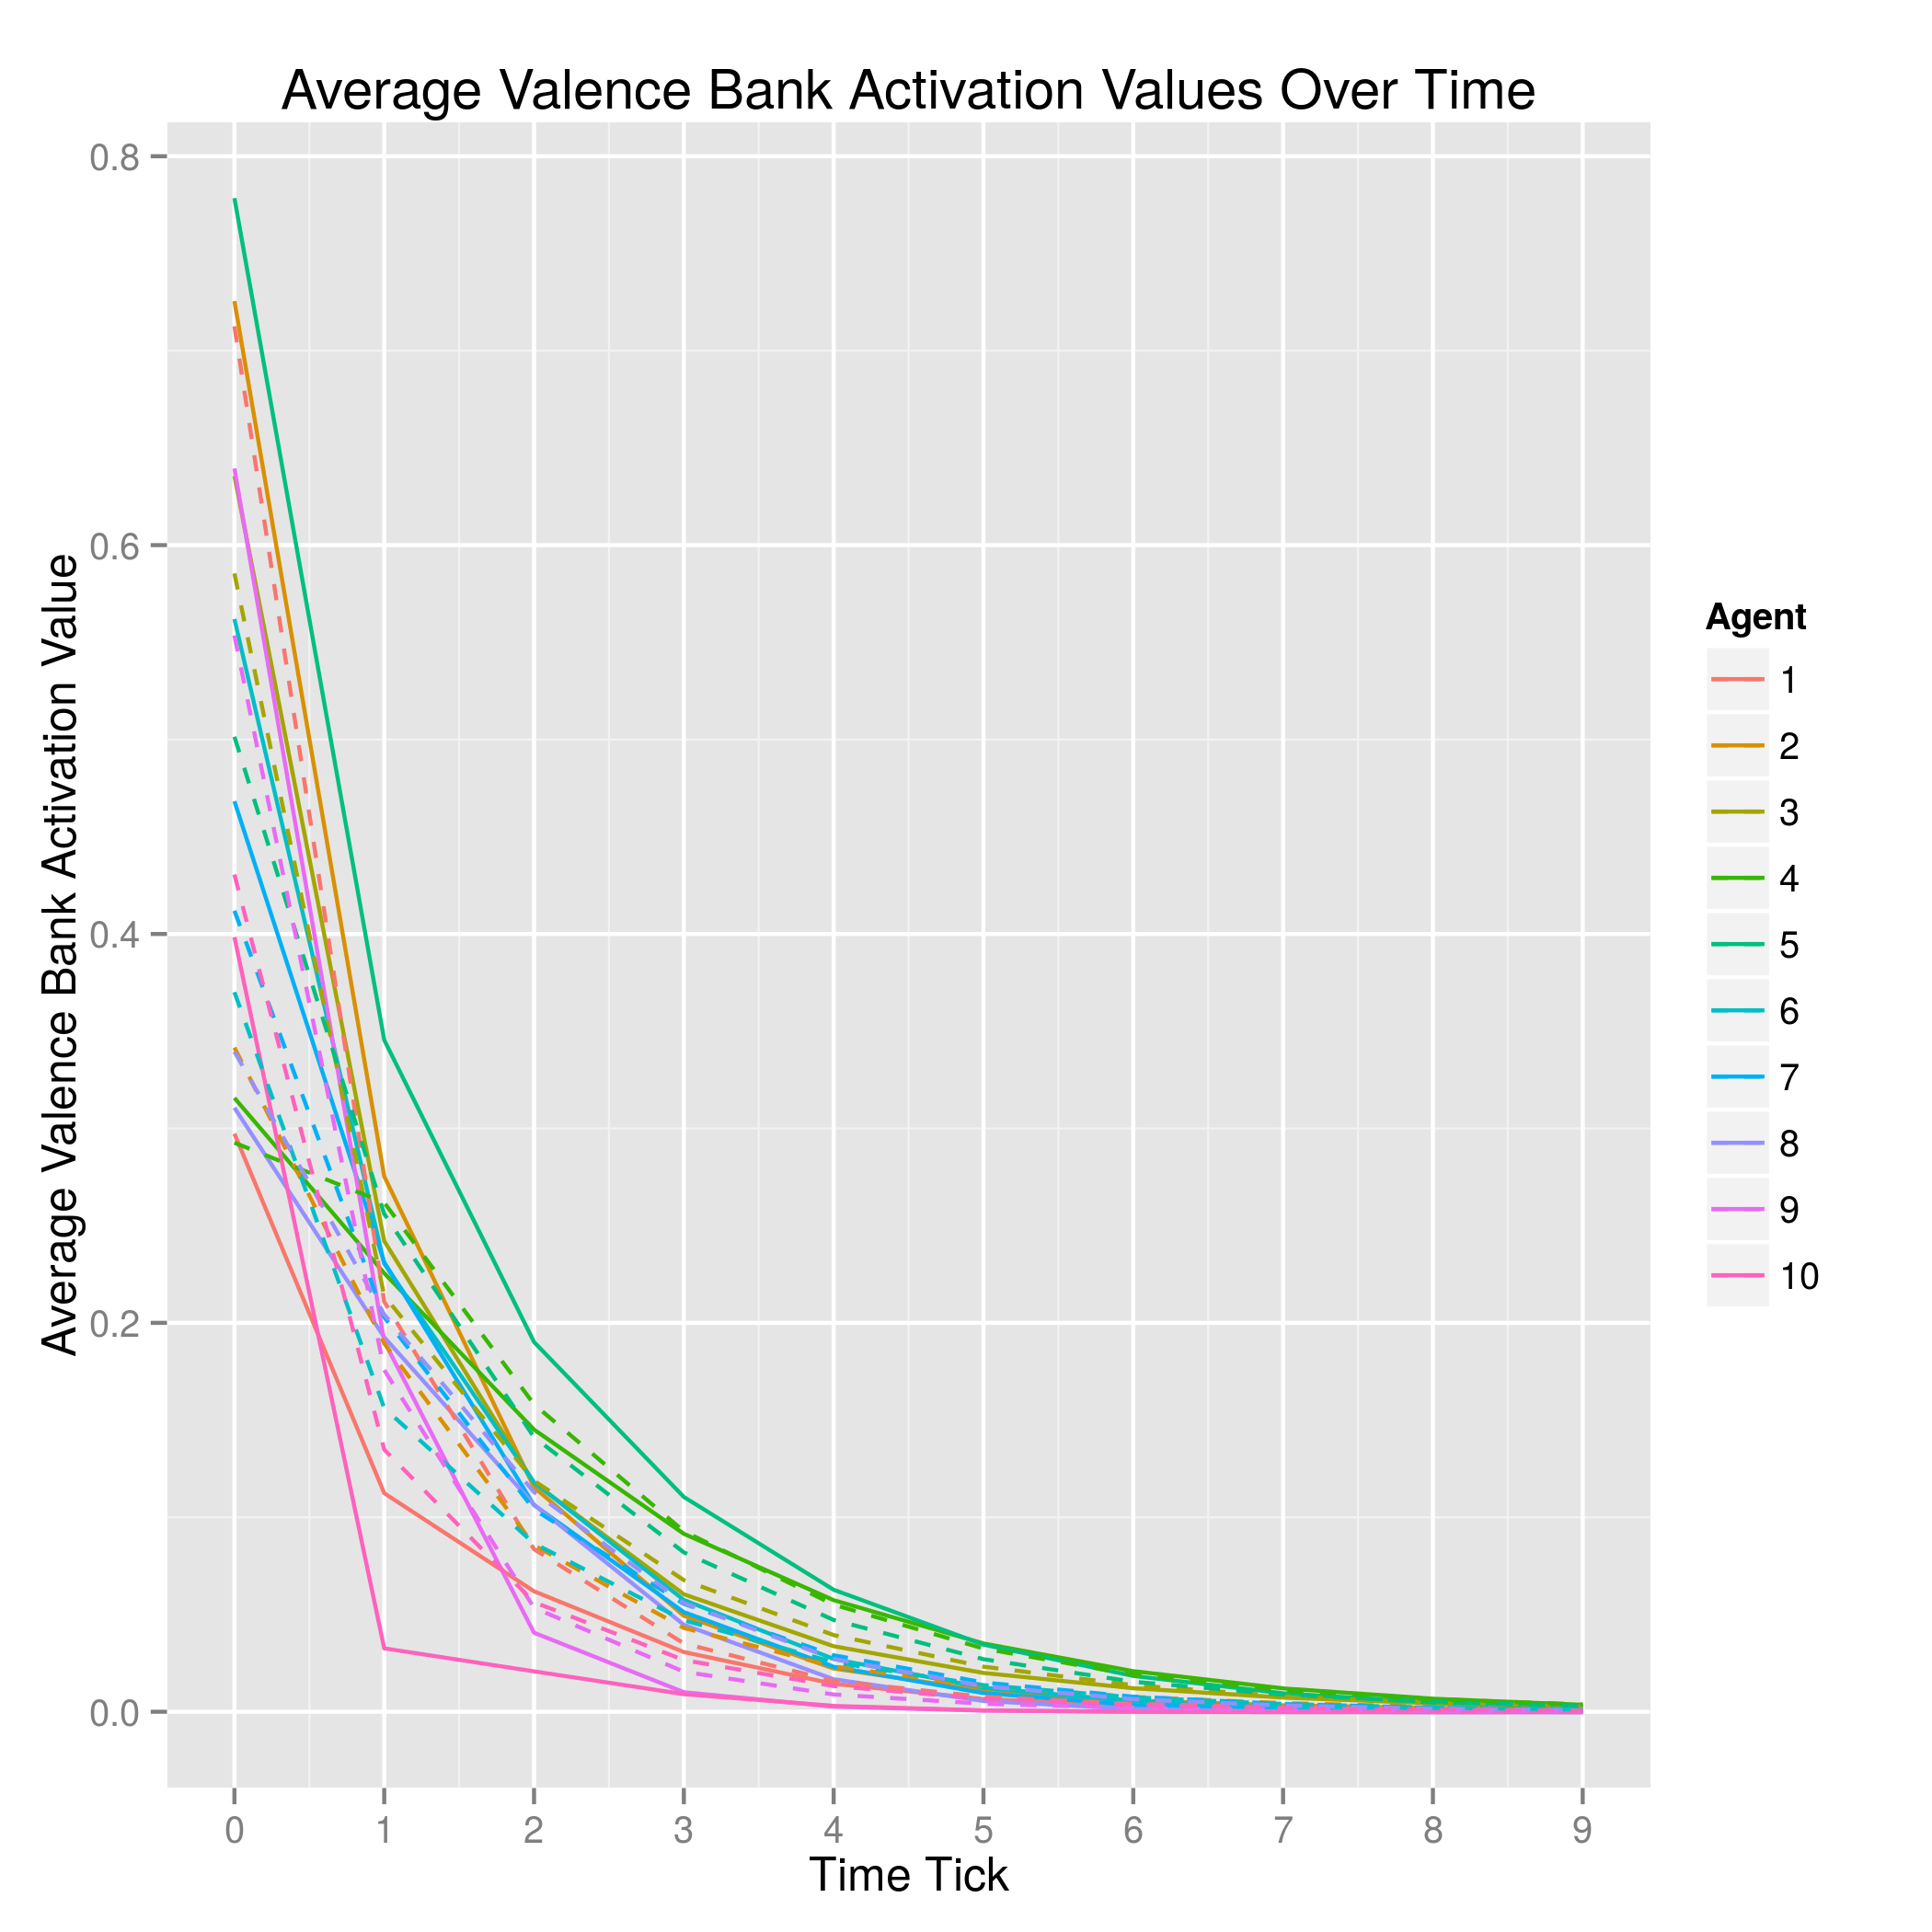
\includegraphics[width=\maxwidth]{figure/plot-sanity-5-v2-nostep} \caption[Sanity Checking 5 with re-implemented edge list, no step]{Sanity Checking 5 with re-implemented edge list, no step\label{fig:plot-sanity-5-v2-nostep}}
\end{figure}


\end{knitrout}


\newpage
\subsection{Sanity 6}
\begin{knitrout}
\definecolor{shadecolor}{rgb}{0.969, 0.969, 0.969}\color{fgcolor}\begin{kframe}
\begin{alltt}
\hlkwd{plot.thesis.data}\hlstd{(}\hlstr{"/home/dchen/git/repast-neural-network-agent-based-model/R/data/sanity6.csv"}\hlstd{,}
    \hlnum{10}\hlstd{,} \hlnum{10}\hlstd{)}
\end{alltt}
\end{kframe}\begin{figure}[]

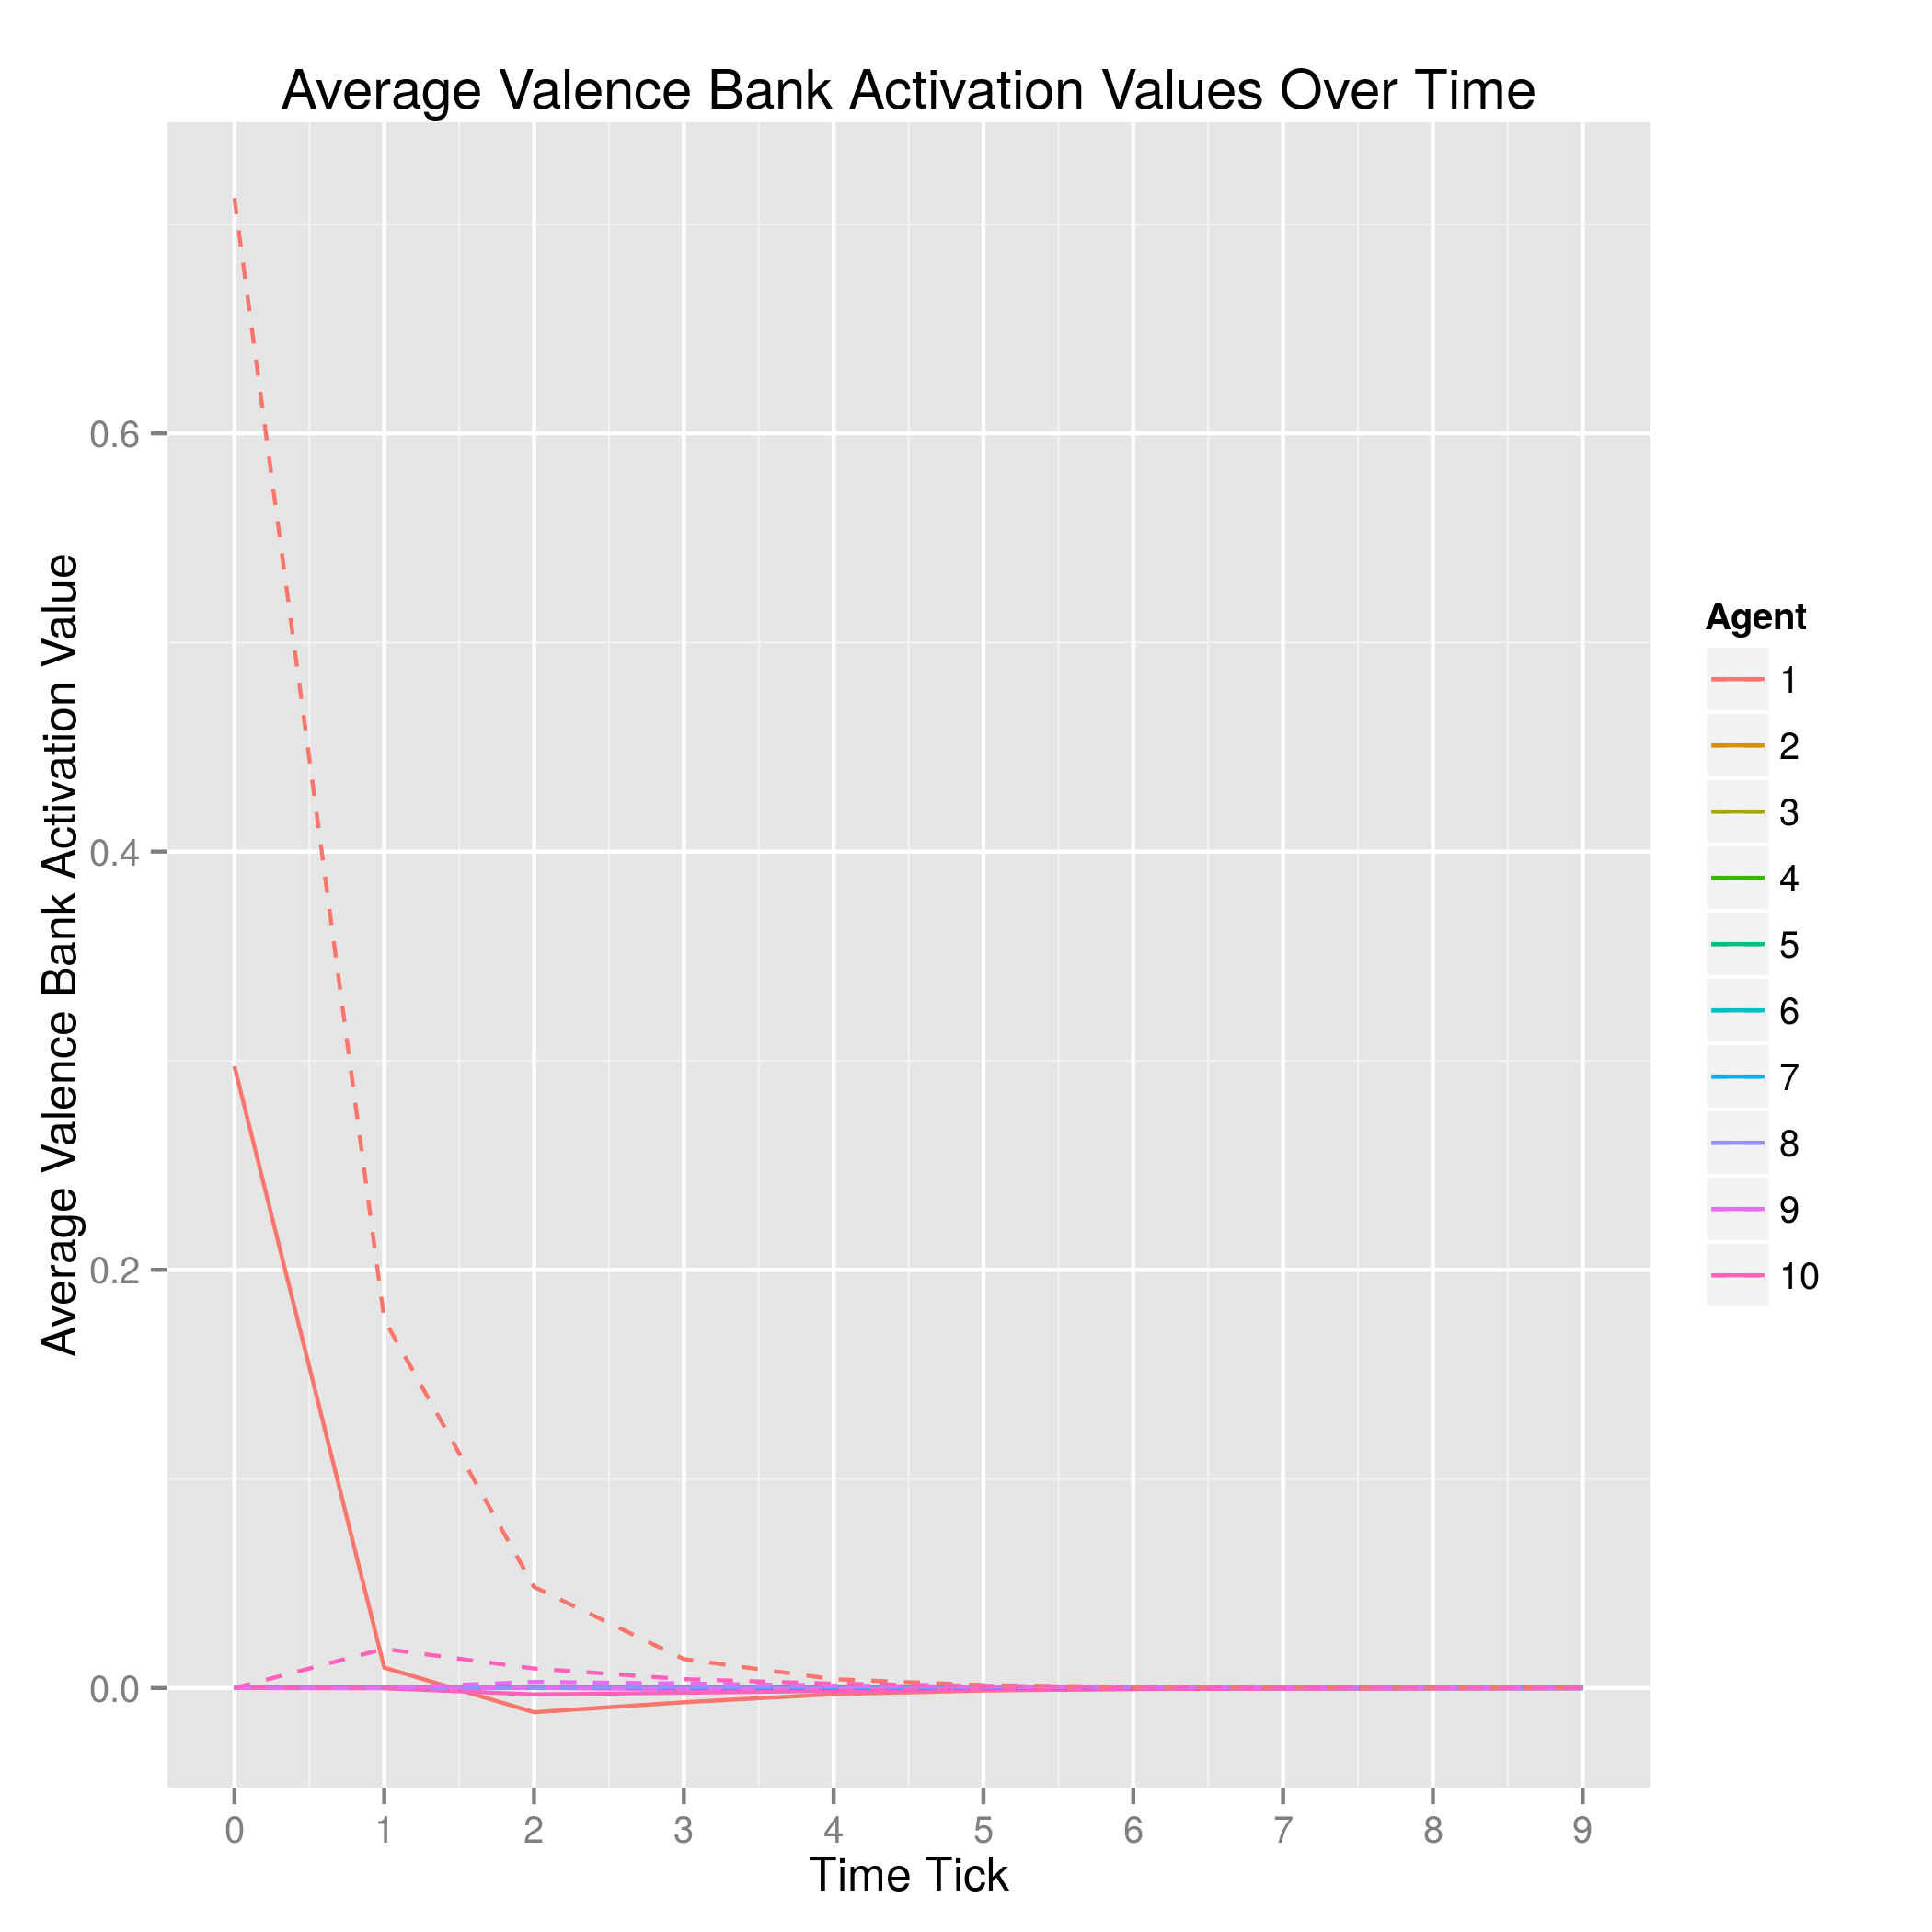
\includegraphics[width=\maxwidth]{figure/plot-sanity-6} \caption[Sanity Checking 6 with re-implemented edge list]{Sanity Checking 6 with re-implemented edge list\label{fig:plot-sanity-6}}
\end{figure}


\end{knitrout}


\newpage
\subsubsection{Sanity 6 no decay}
\begin{knitrout}
\definecolor{shadecolor}{rgb}{0.969, 0.969, 0.969}\color{fgcolor}\begin{kframe}
\begin{alltt}
\hlkwd{plot.thesis.data}\hlstd{(}\hlstr{"/home/dchen/git/repast-neural-network-agent-based-model/R/data/sanity6-nodecay.csv"}\hlstd{,}
    \hlnum{10}\hlstd{,} \hlnum{10}\hlstd{)}
\end{alltt}
\end{kframe}\begin{figure}[]

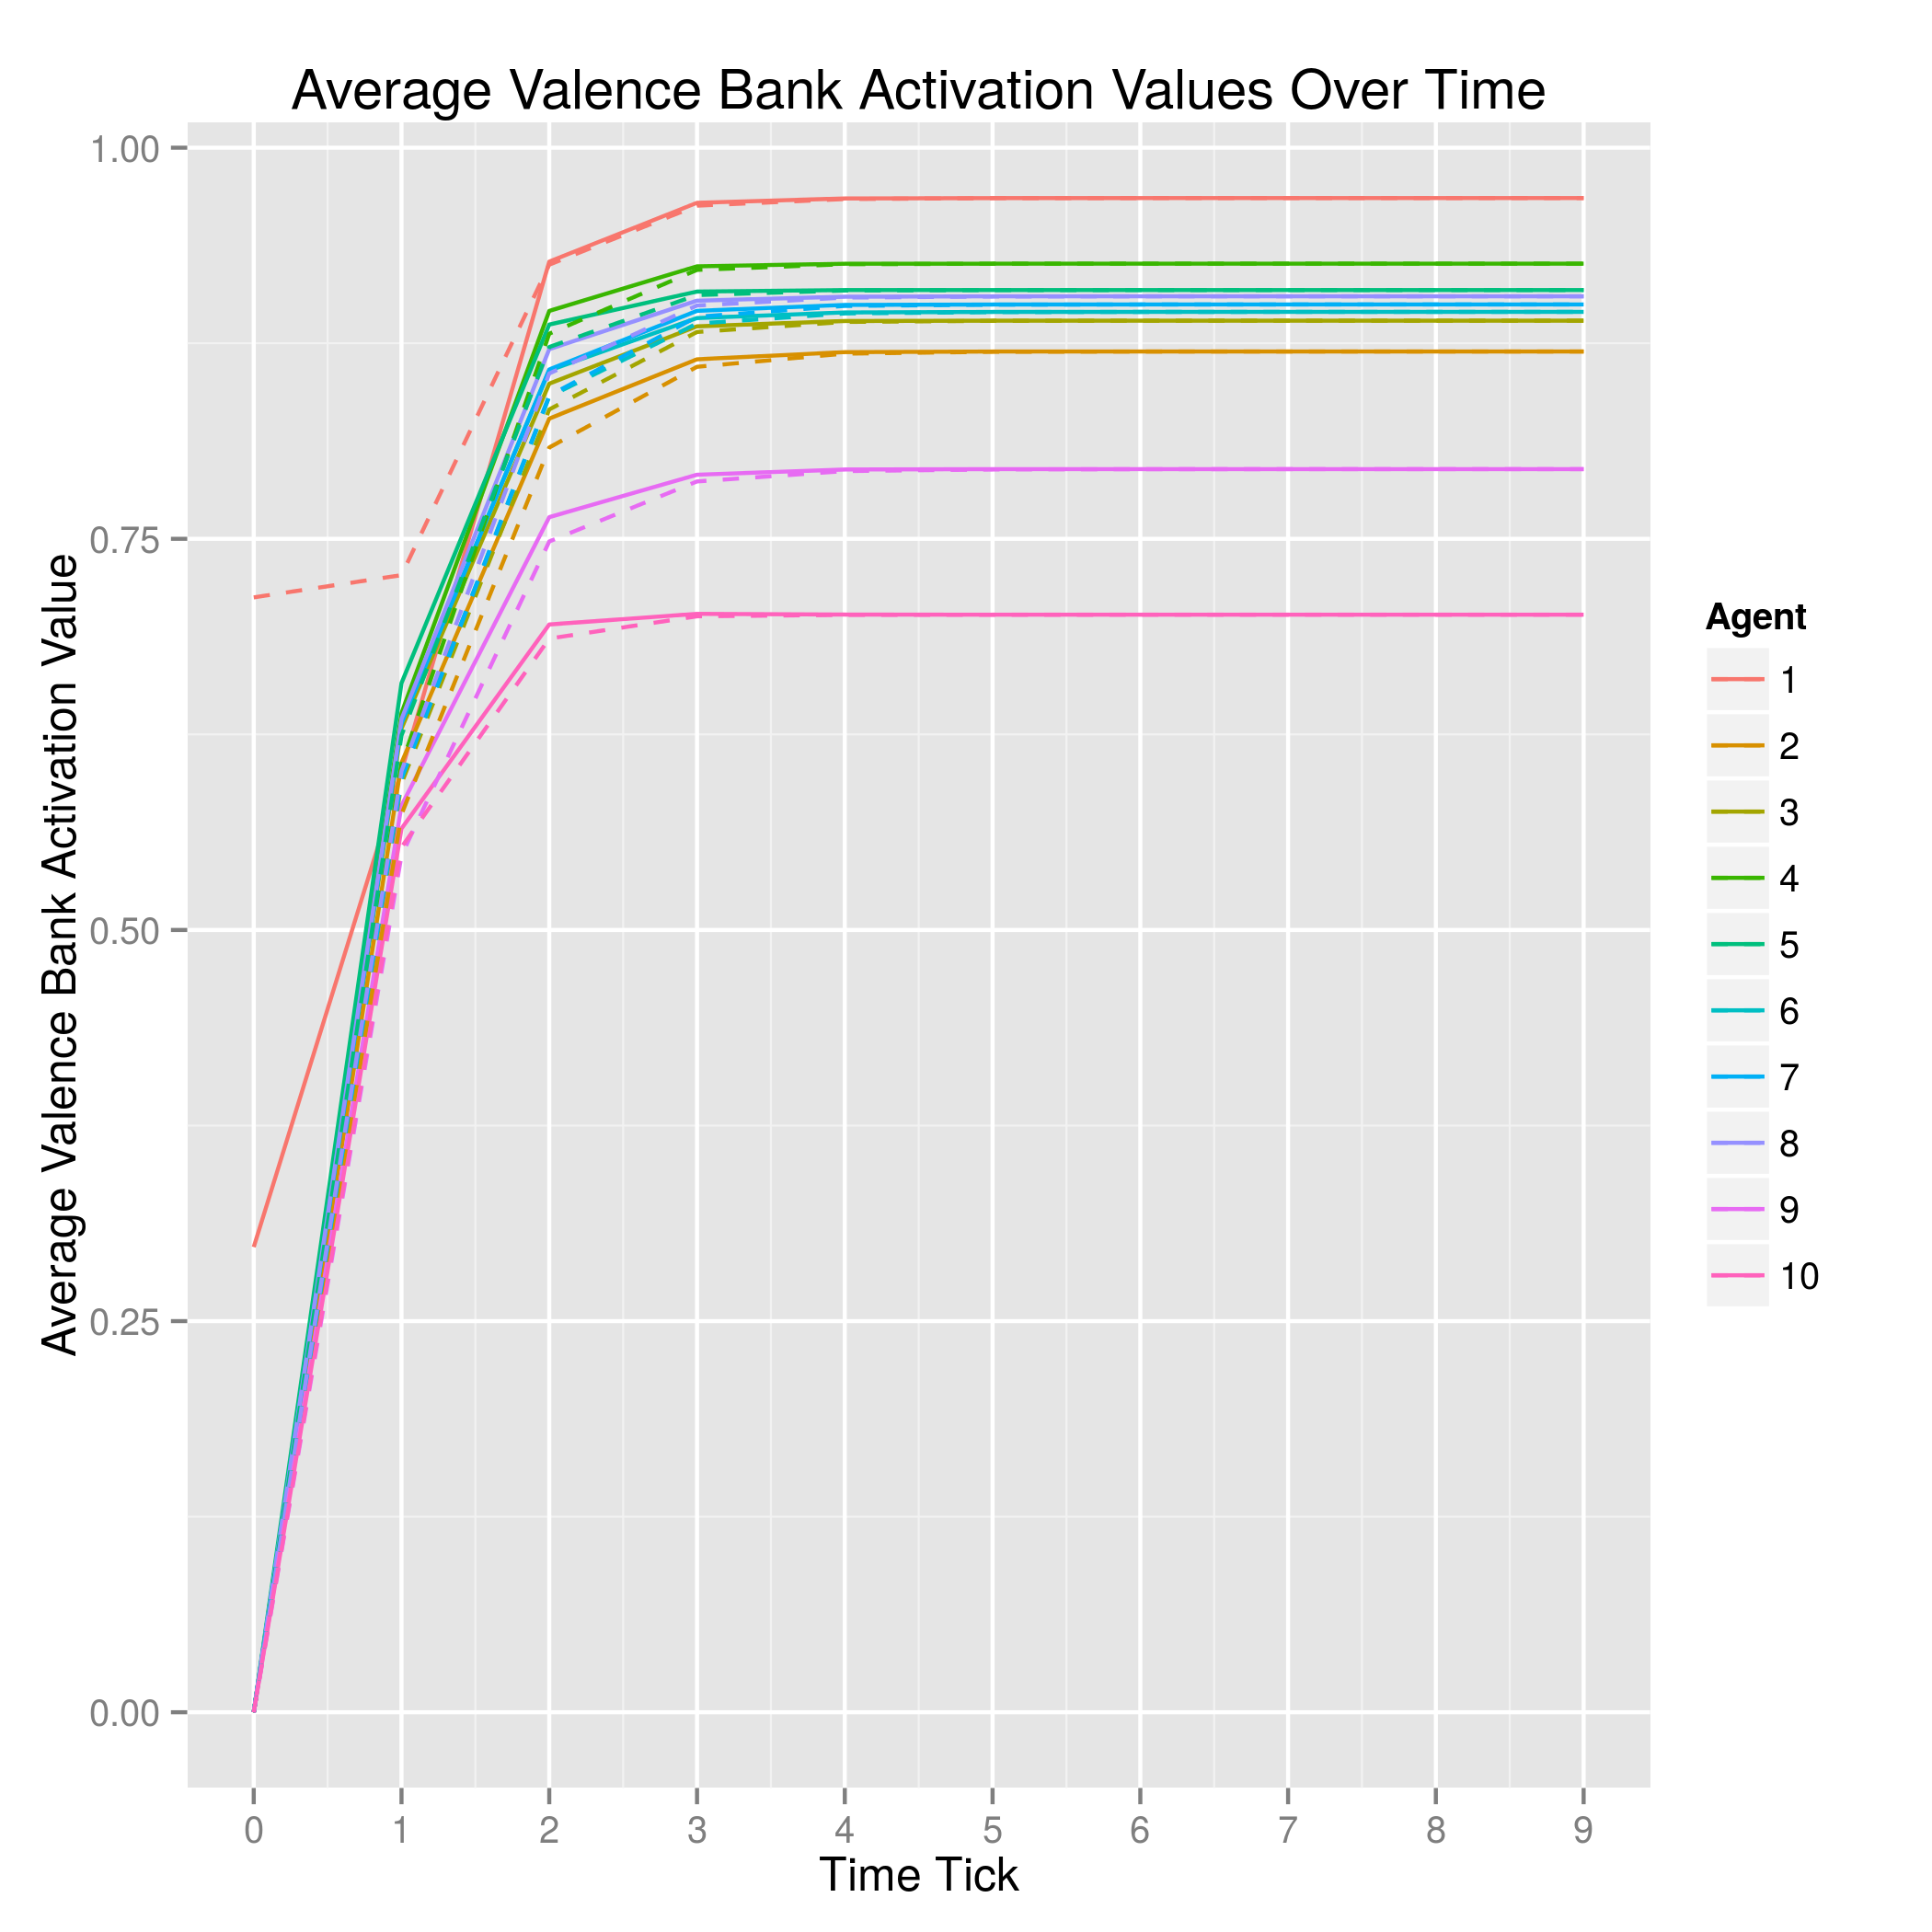
\includegraphics[width=\maxwidth]{figure/plot-sanity-6-nodecay} \caption[Sanity Checking 6 with re-implemented edge list no decay]{Sanity Checking 6 with re-implemented edge list no decay\label{fig:plot-sanity-6-nodecay}}
\end{figure}


\end{knitrout}


\newpage
\subsection{Sanity 7 no decay}
\begin{knitrout}
\definecolor{shadecolor}{rgb}{0.969, 0.969, 0.969}\color{fgcolor}\begin{kframe}
\begin{alltt}
\hlkwd{plot.thesis.data}\hlstd{(}\hlstr{"/home/dchen/git/repast-neural-network-agent-based-model/R/data/sanity7-nodecay.csv"}\hlstd{,}
    \hlnum{10}\hlstd{,} \hlnum{10}\hlstd{)}
\end{alltt}
\end{kframe}\begin{figure}[]

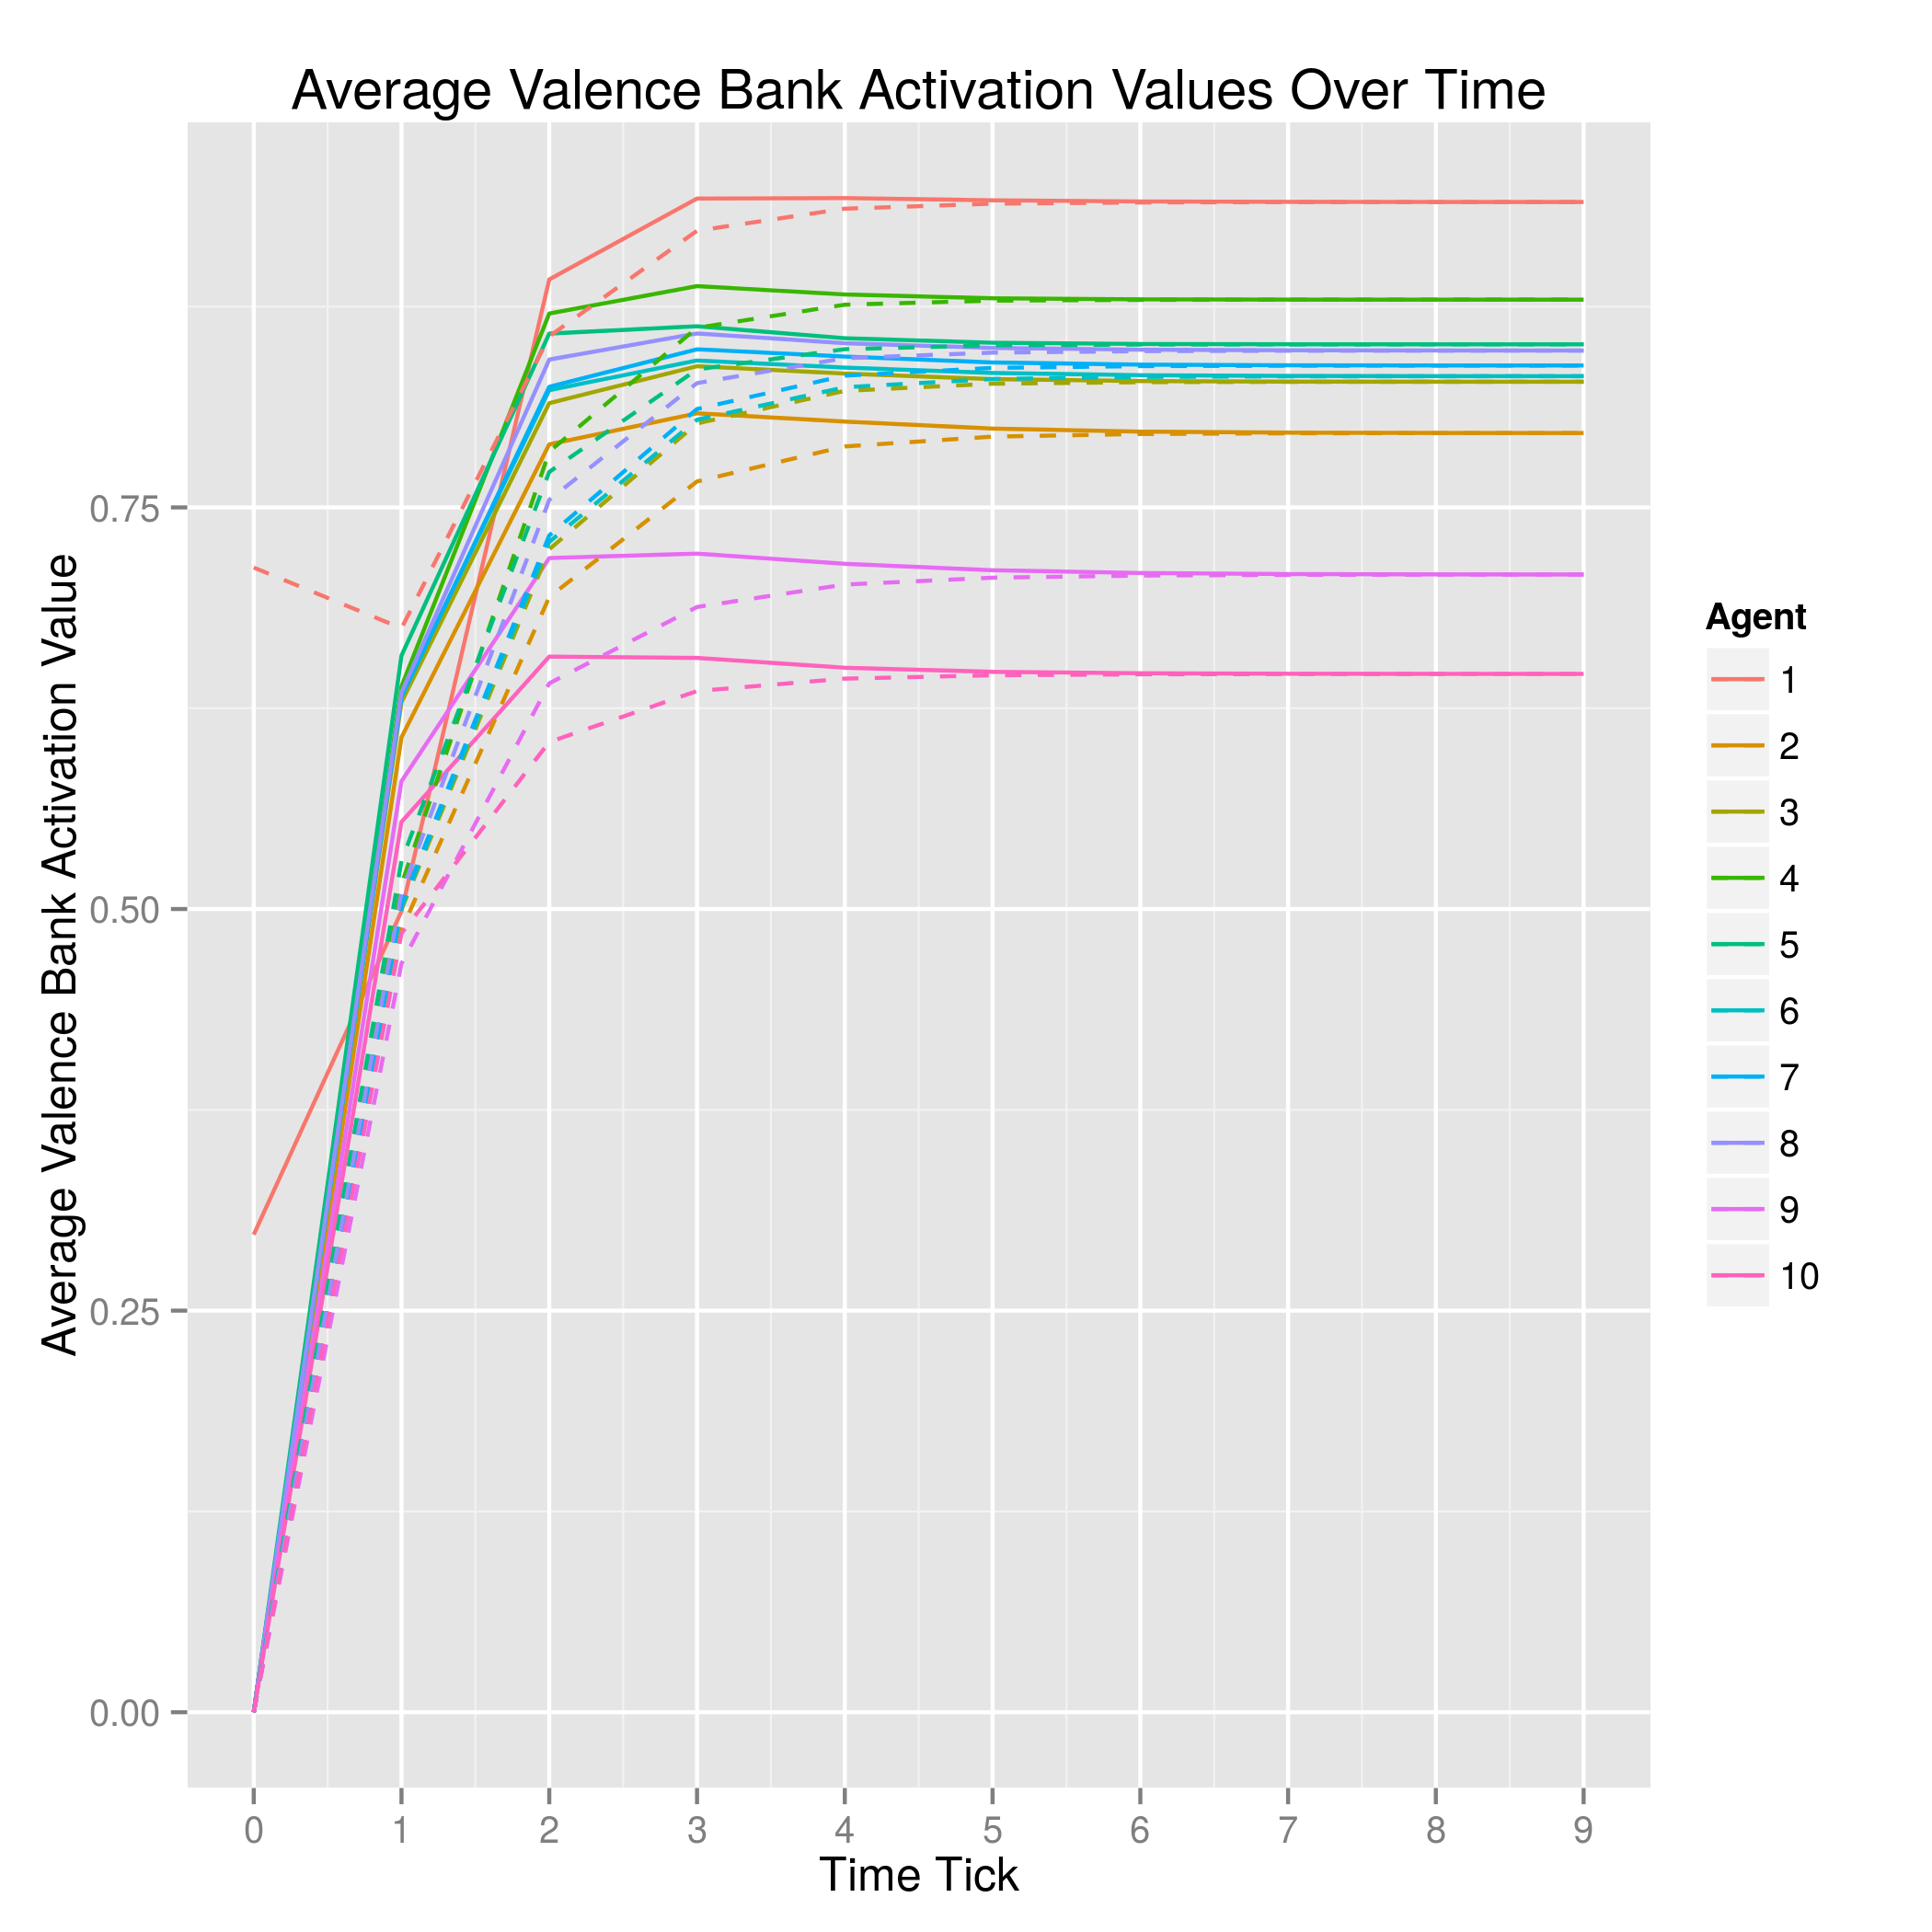
\includegraphics[width=\maxwidth]{figure/plot-sanity-7-nodecay} \caption[Sanity Checking 7 with re-implemented edge list no decay]{Sanity Checking 7 with re-implemented edge list no decay\label{fig:plot-sanity-7-nodecay}}
\end{figure}


\end{knitrout}


\newpage
\section{Output}
\subsection{Output 1}
\label{sec:output1}
Output Data
\begin{itemize}
  \item Agents Activated: 1
  \item Valence Bank: both
  \begin{itemize}
      \item Valence bank activation: random
  \end{itemize}
  \item Valence bank Weights: random
  \begin{itemize}
      \item opposite -0.2
      \item corresponding 0.5
      \item carry over = 0.2
      \item bias = 0
      \item decay = -0.5
  \end{itemize}
  \item Network: circle
  \item Random number: read in from file
  \item Processing units per valence bank: 5
  \item number of agents: 10
  \item number of time ticks: 10,000
\end{itemize}

\subsubsection{First 100 time ticks}
\begin{knitrout}
\definecolor{shadecolor}{rgb}{0.969, 0.969, 0.969}\color{fgcolor}\begin{kframe}
\begin{alltt}
\hlkwd{plot.thesis.data}\hlstd{(}\hlstr{"/home/dchen/git/repast-neural-network-agent-based-model/R/data/agent1-both-random-weights-10k.csv"}\hlstd{,}
    \hlnum{10}\hlstd{,} \hlnum{10000}\hlstd{,} \hlnum{1}\hlstd{,} \hlnum{0}\hlstd{,} \hlnum{100}\hlstd{)}
\end{alltt}
\end{kframe}\begin{figure}[]

\includegraphics[width=\maxwidth]{figure/plot-output-1} \caption[Output 1, first 100 time ticks]{Output 1, first 100 time ticks\label{fig:plot-output-1}}
\end{figure}


\end{knitrout}


\newpage
\subsubsection{All time ticks}
\begin{knitrout}
\definecolor{shadecolor}{rgb}{0.969, 0.969, 0.969}\color{fgcolor}\begin{kframe}
\begin{alltt}
\hlkwd{plot.thesis.data}\hlstd{(}\hlstr{"/home/dchen/git/repast-neural-network-agent-based-model/R/data/agent1-both-random-weights-10k.csv"}\hlstd{,}
    \hlnum{10}\hlstd{,} \hlnum{10000}\hlstd{)}
\end{alltt}
\end{kframe}\begin{figure}[]

\includegraphics[width=\maxwidth]{figure/plot-output-1a} \caption[Output 1, all time ticks]{Output 1, all time ticks\label{fig:plot-output-1a}}
\end{figure}


\end{knitrout}


\newpage
\subsection{Exp1a}
\subsubsection{First 5 time ticks}
\begin{knitrout}
\definecolor{shadecolor}{rgb}{0.969, 0.969, 0.969}\color{fgcolor}\begin{kframe}
\begin{alltt}
\hlkwd{plot.thesis.data}\hlstd{(}\hlstr{"/home/dchen/git/repast-neural-network-agent-based-model/R/data/exp1a.csv"}\hlstd{,}
    \hlnum{40}\hlstd{,} \hlnum{1000}\hlstd{,} \hlnum{1}\hlstd{,} \hlnum{0}\hlstd{,} \hlnum{5}\hlstd{)}
\end{alltt}
\end{kframe}\begin{figure}[]

\includegraphics[width=\maxwidth]{figure/plot-exp1a} \caption[Exp1a, first 100 time ticks]{Exp1a, first 100 time ticks\label{fig:plot-exp1a}}
\end{figure}


\end{knitrout}


\newpage
\subsubsection{All time ticks}
\begin{knitrout}
\definecolor{shadecolor}{rgb}{0.969, 0.969, 0.969}\color{fgcolor}\begin{kframe}
\begin{alltt}
\hlkwd{plot.thesis.data}\hlstd{(}\hlstr{"/home/dchen/git/repast-neural-network-agent-based-model/R/data/exp1a.csv"}\hlstd{,}
    \hlnum{40}\hlstd{,} \hlnum{1000}\hlstd{)}
\end{alltt}
\end{kframe}\begin{figure}[]

\includegraphics[width=\maxwidth]{figure/plot-exp1a1} \caption[Exp1a, all time ticks]{Exp1a, all time ticks\label{fig:plot-exp1a1}}
\end{figure}


\end{knitrout}


\end{document}
